\section{Appendix}
\label{sec:appendix}

\subsection{Experiment Design}
\label{app:experiment-design}

We restate the experimental design and notation used throughout the paper
in a self-contained format here and provide the proofs.

We adopt a generalized fully crossed factorial experimental design.
All independent variables, including language model identity, are treated as factors embedded within a unified design space.

Let $\mathcal{C} = \{1,\dots,C\}$ denote the index set of experimental factors.
Each factor $c \in \mathcal{C}$ admits a finite set of discrete levels, with cardinality $\Lambda_c \in \mathbb{N}$.
We denote the level selected for factor $c$ by
\[
\lambda_c \in \{1,\dots,\Lambda_c\}.
\]
 
The complete experimental design is given by the Cartesian product of the level sets of all factors,
\begin{equation}
\label{eq:design-space}
\mathcal{D}
=
\prod_{c \in \mathcal{C}}
\{1,\dots,\Lambda_c\}.
\end{equation}

For any subset of factors $U \subseteq \mathcal{C}$, we denote
$\boldsymbol{\lambda}_U := (\lambda_c)_{c \in U}$ the vector of factor levels
indexed by $U$.
The vector of the levels for the complete factor set is hence denoted as 
$\boldsymbol{\lambda}_{\mathcal{C}}$ 
(abbreviated as
$\boldsymbol{\lambda}$).



The dependent variable is measured through a psychometric instrument consisting of $K$ items. 
Each item is designed to elicit a response on a shared ordinal scale formalized as an ordered set $(\mathcal{Y}, \preceq)$
\begin{equation}
    \label{eq:Y-support}
    \mathcal{Y} = \{y_{\min}, \dots, y_{\max}\} .
\end{equation}
Each prompt instructs the model to respond with a single digit only (one token) indicating the ordinal category, $\mathcal{Y}$, with no additional text. We therefore treat the model's response as the next-token distribution.

The joint response from all items, $K$, corresponds to a vector 
\begin{equation}
    \label{eq:y-vector}
    \mathbf{y} = (y_1, \dots, y_K) \in \mathcal{Y}^K.
\end{equation}

In behavioral experiments only a subset of the complete output space
corresponds to valid responses. 
Let $\mathcal{V}$ denote the model's full token vocabulary, and let $\mathcal{V}_{\text{val}} \subset {\mathcal{V}}$ denote the set of valid tokens for the task {with the same cardinality as $\mathcal{Y}$, $|\mathcal{V}_{\text{val}}|=|\mathcal{Y}|$}. 
Let $P_{\text{raw}}(t \mid x)$ denote the model's next-token probability distribution given a prompt $x$, defined over the full vocabulary {$\mathcal{V}$}. We define the valid probability mass as
\begin{equation}
    P_{\text{val}}(x) = \sum_{t \in \mathcal{V}_{\text{val}}} P_{\text{raw}}(t \mid x).    
\end{equation}

To interface with the language model, we define a surjective mapping 
\begin{equation}
    \label{eq:phi}
\phi: \mathcal{V}_{\text{val}} \to \mathcal{Y}    
\end{equation}
that accounts for tokenizer-specific variations of digits (e.g., leading spaces) and associates a specific subset of valid vocabulary tokens $\mathcal{V}_{\text{val}} \subset {\mathcal{V}}$ with their numeric values, $\mathcal{Y}$.
This mapping transforms the token distribution into a probability mass function over ordinal integers, allowing us to use ordinal dispersion measures to calculate the internal consistency of the model's predictive distribution.

\subsection{Conditional Independence via Context Isolation}
\label{sec:independence-assumption}

A central property of this design is that the model's internal state is reset between items. For a fixed experimental condition $\boldsymbol{\lambda}$, the response $Y_{k,\boldsymbol{\lambda}}$ for item $k$ depends solely on the specific prompt $x_{k,\boldsymbol{\lambda}}$ and the model parameters. 
Following \citet{wadi2025a}, we treat the items as conditionally independent given $\boldsymbol{\lambda}$.
Formally, for any realization vector $\mathbf{y} \in \mathcal{Y}^K$, the joint probability mass function factorizes as
\begin{equation}
\label{eq:joint-distribution-app}
    P(\mathbf{Y}_{\boldsymbol{\lambda}} = \mathbf{y} \mid \boldsymbol{\lambda}) = \prod_{k=1}^{K} P(Y_{k,\boldsymbol{\lambda}} = y_k \mid \boldsymbol{\lambda}).
\end{equation}
This assumption justifies the use of product measures for joint distributions (Appendix \ref{app:consensus}) and convolution for composite sums (Appendix \ref{app:construct}).

\subsection{The Consensus Layer}
\label{app:consensus}
Having confirmed the model's focus on valid outputs, 
we now superimpose the numeric, ordinal structure of the task 
onto the analysis. 
We require a measure that quantifies whether the model's attitude towards the numeric scale is behaviorally consistent. Consider a single item with a $7$-point Likert scale ($\mathcal{Y}=\{1,\dots,7\}$). A distribution assigning equal mass to opposing endpoints with the following probability mass functions (PMFs)
\[
P(Y=1)=0.5, \quad P(Y=7)=0.5,
\]
exhibits dissension, as the model simultaneously expresses diametrically opposing views. In contrast, a distribution concentrated on adjacent scale points,
\[
P(Y=5)=0.5, \quad P(Y=6)=0.5,
\]
is logically consistent, reflecting only local uncertainty regarding the precise intensity of the attitude.


% consensus table
\begin{table}[t]
  \caption{Visualization of LLM Consensus (Cns) and Dissension (Dsn) cases. Each histogram depicts a characteristic output distribution on a 1--7 scale.}
  \label{tab:consensus-dissension-visual}
  \begin{center}
    \begin{small}
      \begin{sc}
        % Using 'c' for numbers and 'm' for images to ensure vertical centering
        \begin{tabular}{ccm{2.7cm}}
          \toprule
          Cns & Entropy & \multicolumn{1}{c}{Distribution} \\
          \midrule
          1.00 & 0.00 & 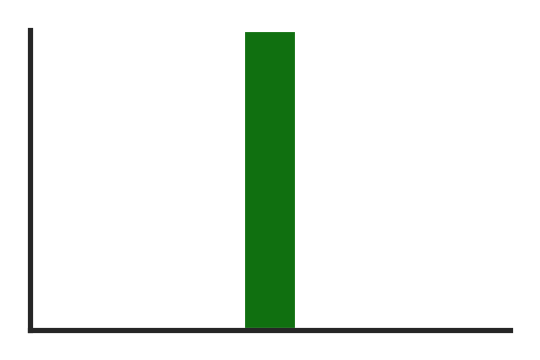
\includegraphics[width=\linewidth]{figures/hist_4.png} \\
          
          0.84 & 1.57 & 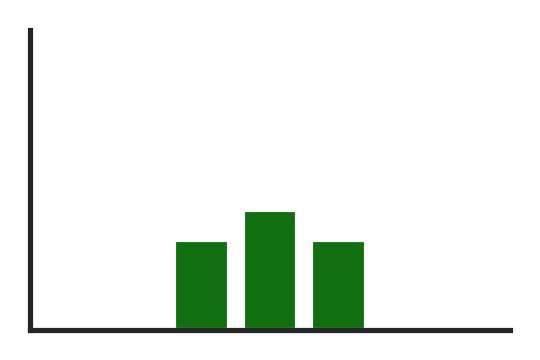
\includegraphics[width=\linewidth]{figures/hist_3,4,5.png} \\
          
          0.47 & 2.81 & 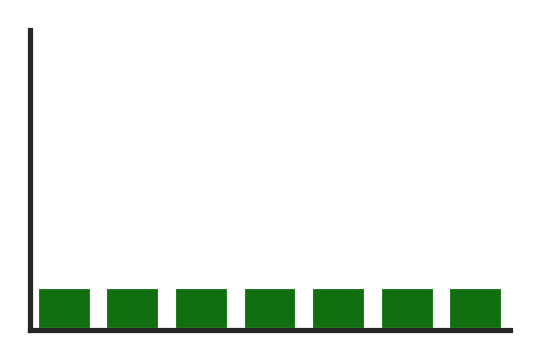
\includegraphics[width=\linewidth]{figures/hist_1,2,3,4,5,6,7.png} \\
          
          0.74 & 1.00 & 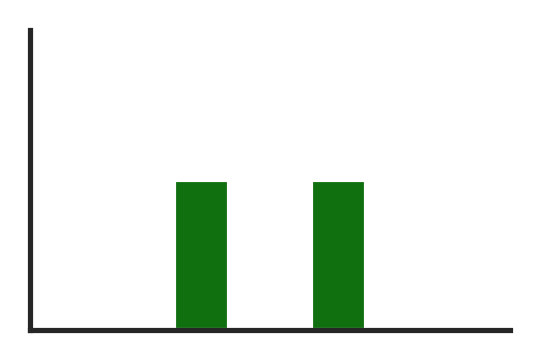
\includegraphics[width=\linewidth]{figures/hist_3,5.png} \\

          0.00 & 1.00 & 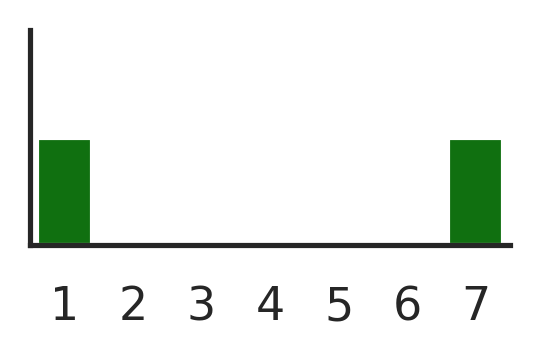
\includegraphics[width=\linewidth]{figures/hist_1,7.png} \\
          \bottomrule
        \end{tabular}
      \end{sc}
    \end{small}
  \end{center}
  \vskip -0.1in
\end{table}


To obtain a measure of consensus from a sample of individuals, 
\citet{tastle2007consensus} introduced Consensus ($\mathrm{Cns}$) as
\begin{equation}
    \small 
    \label{eq:consensus-original}
        \mathrm{Cns}(Y) = 1 + \sum_{y \in \mathcal{Y}} \biggl[ P(Y=y) \times \log_2 \left( 1 - \frac{|y - \mu_Y|}{d_{\max}} \right) \biggr]
\end{equation}
where $\mu_Y = \sum_{y \in \mathcal{Y}} y P(Y=y)$ is the expected value of the ordinal distribution and $d_{\max} =  y_{\max} - y_{\min}$.
Table \ref{tab:consensus-dissension-visual} illustrates Consensus on different PMFs.
The issue with using entropy to measure consensus is shown in the 4th 
($P(3)=0.5$ and $P(5)=0.5$) 
and 5th row 
($P(1)=0.5$ and $P(7)=0.5$), 
where the latter shows lower levels of consensus, but entropy gives the same value
($Entropy=1.00$).




Whereas the original Consensus statistic is defined over a sample
of aggregated scalar responses,
our setting differs in two fundamental ways.
First, with language models as subjects, we have direct access to the PMF
of the data generation process rather than sampled responses.
Second, behavioral instruments such as Likert scales typically consist of
multiple items, each with varying levels of Consensus and Dissension.
Calculating Consensus over aggregated responses
disregards the inter-item Dissension.

% consensus-original-issue
\begin{figure}[t]
    \includegraphics[width=\columnwidth]{figures/consensus-original-issue.pdf}
    \caption{
    The failure of aggregate Consensus in capturing between-item dissension.
    Distinct response patterns in a two-item Likert space
    (e.g., $(4,4)$ vs.\ $(1,7)$)
    collapse to the same scalar score after aggregation.
    The original Consensus measure operates on this projection
    and cannot detect between-item dissension.
    }
    \label{fig:consensus-original-issue}
\end{figure}
 

Standard aggregation procedures, 
such as summation or averaging,
project this space onto a single scalar dimension. 
Figure~\ref{fig:consensus-original-issue} illustrates this effect for a two-item, 7-point Likert scale. Response patterns such as $(4,4)$, $(1,7)$, and $(7,1)$ all yield the same aggregate sum, causing the inter-item Dissension to be lost. However, these points occupy very different locations in the original two-dimensional response space, with $(1,7)$ and $(7,1)$ representing maximal disagreement between items.

Thus, we derive the Multivariate Consensus (Consensus from now on) across all items on a common ordinal scale. 
For each item $k \in \{1,\dots,K\}$, we utilize the mapping $\phi$ (Eq.~\ref{eq:phi}) to project the renormalized token distribution onto the ordinal scale $\mathcal{Y}$ (Eq.~\ref{eq:y-vector}). We define the item-level ordinal random variable $Y_k$ with probability mass function

\begin{equation}
\label{eq:phi-inverse-mapping}
    P(Y_k = y) = P\left(t = \phi^{-1}(y) \mid x_k, t \in \mathcal{V}_{\text{val}}\right),
\end{equation}
where $x_k$ is the prompt for item $k$. This step formally converts the model's token prediction into a numeric behavioral response.
% Since items are elicited via independent prompts (Sec.~\ref{sec:independence-assumption}), 
% the item-wise distributions are independent. 
% This allows us to use the joint random vector $\mathbf{Y} = (Y_1, \dots, Y_K)$ with probability mass function in Eq.~\ref{eq:joint-distribution}.
We compute the expected response for each item, forming the centroid of the joint distribution
\begin{equation}
\label{eq:centroid}
    \boldsymbol{\mu} = (\mu_1, \dots, \mu_K),
\end{equation}
where $\mu_k = \sum_{y \in \mathcal{Y}} y P(Y_k = y)$.
The centroid, $\boldsymbol{\mu}$, represents the model's expected position on each Likert item in the $K$-dimensional space. We define the maximum possible distance between any response vector and the centroid as the diagonal of the hypercube defined by the scale extrema
\begin{equation}
\label{eq:d-max}
    d_{\max} = \sqrt{K \,(y_{\max} - y_{\min})^2}.
\end{equation}

This normalizes distances to the unit interval and ensures comparability across instruments with different numbers of items. The Multivariate Consensus is defined as the expected logarithmic agreement of the joint distribution with respect to the centroid (Eq.~\ref{eq:consensus-multivariate}).



Intuitively, this measure assigns higher consensus when the probability mass is concentrated near the centroid across all items, and lower consensus when mass is dispersed or polarized. Unlike entropy-based measures, Consensus is sensitive to ordinal distances. When $K=1$, the multivariate formulation reduces to the original Consensus \citep{tastle2007consensus}, with the key distinction that we operate directly on the true PMF rather than on sampled responses.
Multivariate Dissension ($\mathrm{Dsn}$) is defined as 
the complement of Consensus, 
representing the degree of polarization or 
dispersion away from the mean.

\begin{equation}    
\label{eq:dissension}
\begin{aligned}
\mathrm{Dsn}(\mathbf{Y}) = 1 - \mathrm{Cns}(\mathbf{Y})
\end{aligned}
\end{equation}


\subsection{The Construct Layer}
\label{app:construct}

Our goal is to quantify differences in the dependent variable across
experimental conditions and models, while fully propagating
uncertainty induced by the model's generative process. 
We formalize inference over latent scale scores
using an analytical fixed-effects ANOVA/Hoeffding decomposition.
For a specific condition vector $\boldsymbol{\lambda}$, 
the composite scale score, $S_{\boldsymbol{\lambda}}$, 
is the aggregation of item-level random variable responses

\begin{equation}
\label{eq:s-lambda}
S_{\boldsymbol{\lambda}}
=
\sum_{k=1}^K Y_{k,\boldsymbol{\lambda}}.
\end{equation}

Let $P_{Y_{k, \boldsymbol{\lambda}}}$ denote the PMF of item $k$ under condition $\boldsymbol{\lambda}$. Given independence (Sec.~\ref{sec:independence-assumption}), the distribution of the composite score is obtained via discrete convolution
\begin{equation}
\label{eq:item-wise-convolution}
    P_{S_{\boldsymbol{\lambda}}} = P_{Y_{1, \boldsymbol{\lambda}}} \circledast P_{Y_{2, \boldsymbol{\lambda}}} \circledast \dots \circledast P_{Y_{K, \boldsymbol{\lambda}}}.
\end{equation}
 

\subsubsection{Factorial Decomposition Over Distributions}

We formalize an analytical ANOVA/Hoeffding decomposition of the composite scale score. 
Our framework constructs a unique family of centered effect distributions $\{E_U\}_{U \subseteq \mathcal{C}}$, representing main effects and interactions, such that the total expected score satisfies the additive identity
\begin{equation}
\label{eq:decomposition-preview}
\small
\mathbb{E}[S_{\boldsymbol{\lambda}}] = \underbrace{\mathbb{E}[S_0]}_{\text{Grand Mean}} + \sum_{c \in \mathcal{C}} \underbrace{\mathbb{E}[E_c(\lambda_c)]}_{\text{Main Effects}} + \sum_{\substack{U \subseteq \mathcal{C} \\ |U| \ge 2}} \underbrace{\mathbb{E}[E_U(\boldsymbol{\lambda}_U)]}_{\text{Interactions}},
\end{equation}

while retaining the full probability mass function for every term in the summation.

For each experimental condition  
\(\boldsymbol{\lambda} \in \mathcal{D}\), the composite scale score
$S_{\boldsymbol{\lambda}}$ 
is a discrete random variable with probability mass function
\(P_{S_{\boldsymbol{\lambda}}}\) (Eq.~\ref{eq:s-lambda}).
Rather than reducing \(S_{\boldsymbol{\lambda}}\) to a point estimate,
we treat the mapping
\begin{equation}
\boldsymbol{\lambda}
\;\mapsto\;
P_{S_{\boldsymbol{\lambda}}}    
\end{equation}

as the primitive object of analysis.  
This allows all uncertainty induced by the model's generative process to be propagated exactly through subsequent analyses.
Given the fully crossed factorial design, 
all factor combinations are symmetric.
Therefore, 
the design space $\mathcal{D}$ takes on a uniform probability
distribution $\pi$, 
assigning equal weight
to each experimental condition.

\begin{assumption}[Fully Crossed Fixed-Effects Design]
\label{ass:fully-crossed}
The experimental design space
\(
\mathcal{D} = \prod_{c \in \mathcal{C}} \{1,\dots,\Lambda_c\}
\)
is finite and fully crossed. All expectations over
\(\mathcal{D}\) are taken with respect to the uniform measure.
\end{assumption}


\begin{proposition}[Linearity of Expectation under Mixture Marginalization]
\label{prop:linearity-mixture}
Let $\mathcal{D}$ be a finite factorial design with probability measure $\pi$, and let $P_{\bar S} = \mathbb{E}_{\boldsymbol{\lambda} \sim \pi} [P_{S_{\boldsymbol{\lambda}}}]$ be the mixture distribution. Then,
\begin{equation}
\label{eq:mixture-expectation}
\mathbb{E}[\bar S]
=
\mathbb{E}_{\boldsymbol{\lambda} \sim \pi}
\!\left[
\mathbb{E}[S_{\boldsymbol{\lambda}}]
\right].
\end{equation}
\end{proposition}

The proof follows immediately from the linearity of finite sums and the definition of expectation.


\begin{corollary}[Expectation of Factorial Marginal Distributions]
\label{cor:anova-consistency}
Let $S_U(\boldsymbol{\lambda}_U)$ denote a factorial
marginal distribution defined by marginalizing $P_{S_{\boldsymbol{\lambda}}}$ over
$\boldsymbol{\lambda}_{-U}$ under the uniform measure.
Then
\[
\mathbb{E}\!\left[S_U(\boldsymbol{\lambda}_U)\right]
=
\mathbb{E}_{\boldsymbol{\lambda}_{-U}}
\!\left[
\mathbb{E}[S_{\boldsymbol{\lambda}}]
\right].
\]
\end{corollary}


The proof follows directly from Prop.~\ref{prop:linearity-mixture}
by taking $\pi$ to be the uniform distribution over
$\boldsymbol{\lambda}_{-U}$.


\subsubsection{Grand Mixture Distribution}

To establish a baseline for factorial effects, we construct the distributional equivalent of the classical ANOVA Grand Mean. We compute this as the Grand Mixture Distribution ($P_{S_0}$), obtained by averaging the composite score distributions uniformly across the entire design space $\mathcal{D}$
\begin{equation}
\label{eq:grand-mixture}
P_{S_0}
=
\mathbb{E}_{\boldsymbol{\lambda} \sim \pi}
\!\left[
P_{S_{\boldsymbol{\lambda}}}
\right]
=
\frac{1}{|\mathcal{D}|}
\sum_{\boldsymbol{\lambda} \in \mathcal{D}}
P_{S_{\boldsymbol{\lambda}}}.  
\end{equation}


The random variable \(S_0\) encapsulates the global background distribution of the construct, encompassing all sources of variation in the experiment.



\subsubsection{Marginal Distributions}
\label{app:marginal-slices}

ANOVA Marginal Mean averages responses over complementary factors to isolate a specific level. We extend it by computing the Marginal Slice Distribution ($P_{M_c(\lambda_c)}$). This is obtained by taking the uniform mixture of composite score distributions over all factors other than $c$,

{\small
\begin{equation}
\label{eq:marginal-means}
\small
\begin{split}
P_{M_c(\lambda_c)}&=\mathbb{E}_{\boldsymbol{\lambda}_{-c}}\!\left[P_{S_{(\lambda_c,\boldsymbol{\lambda}_{-c})}}\right]\\
                  &=\frac{1}{|\mathcal{D}_{-c}|}\sum_{\boldsymbol{\lambda}_{-c}\in\mathcal{D}_{-c}}P_{S_{(\lambda_c,\boldsymbol{\lambda}_{-c})}}.
\end{split}
\end{equation}
}

The random variable \(M_c(\lambda_c)\) is the predictive distribution of the
composite score when factor \(c\) is fixed at level \(\lambda_c\), averaging
uniformly over all remaining factors. 
At the expectation level (Prop.~\ref{prop:linearity-mixture}),
\(\mathbb{E}[M_c(\lambda_c)]\) equals the classical marginal mean.

\begin{corollary}[Grand mixture as an average of marginal slices]
\label{cor:grand-as-average-of-marginals}
Under Assumption~\ref{ass:fully-crossed}, for any factor \(c\),
\begin{equation}
\label{eq:grand-as-average-of-marginals}
P_{S_0}
=
\frac{1}{\Lambda_c}
\sum_{\lambda_c=1}^{\Lambda_c}
P_{M_c(\lambda_c)}.
\end{equation}
\end{corollary}

\begin{proof}
Fix \(c \in \mathcal{C}\). The grand mixture distribution is
\begin{equation}
\label{eq:proof-grand-def}
P_{S_0}
=
\frac{1}{|\mathcal{D}|}
\sum_{\boldsymbol{\lambda}\in\mathcal{D}}
P_{S_{\boldsymbol{\lambda}}}.
\end{equation}
Under Assumption~\ref{ass:fully-crossed}, the design space factors as
\(
\mathcal{D} \;=\; \{1,\dots,\Lambda_c\}\times \mathcal{D}_{-c},
\)
where
\(
\mathcal{D}_{-c} := \prod_{d\in\mathcal{C}\setminus\{c\}}\{1,\dots,\Lambda_d\}.
\)
Hence each \(\boldsymbol{\lambda}\in\mathcal{D}\) can be written uniquely as
\(\boldsymbol{\lambda}=(\lambda_c,\boldsymbol{\lambda}_{-c})\) with
\(\lambda_c\in\{1,\dots,\Lambda_c\}\) and \(\boldsymbol{\lambda}_{-c}\in\mathcal{D}_{-c}\).
We may rewrite the sum in Eq.~\eqref{eq:proof-grand-def} as a double sum
\begin{equation}
\label{eq:proof-double-sum}
P_{S_0}
=
\frac{1}{|\mathcal{D}|}
\sum_{\lambda_c=1}^{\Lambda_c}
\sum_{\boldsymbol{\lambda}_{-c}\in\mathcal{D}_{-c}}
P_{S_{(\lambda_c,\boldsymbol{\lambda}_{-c})}}.
\end{equation}
Because the design is fully crossed,
\(
|\mathcal{D}| = \Lambda_c \, |\mathcal{D}_{-c}|.
\)
Substituting this into Eq.~\eqref{eq:proof-double-sum} gives

{\small
\begin{align}
P_{S_0}
&=
\frac{1}{\Lambda_c\,|\mathcal{D}_{-c}|}
\sum_{\lambda_c=1}^{\Lambda_c}
\sum_{\boldsymbol{\lambda}_{-c}\in\mathcal{D}_{-c}}
P_{S_{(\lambda_c,\boldsymbol{\lambda}_{-c})}}
\label{eq:proof-factor-cardinality}\\[4pt]
&=
\frac{1}{\Lambda_c}
\sum_{\lambda_c=1}^{\Lambda_c}
\left(
\frac{1}{|\mathcal{D}_{-c}|}
\sum_{\boldsymbol{\lambda}_{-c}\in\mathcal{D}_{-c}}
P_{S_{(\lambda_c,\boldsymbol{\lambda}_{-c})}}
\right).
\label{eq:proof-recognize-marginal}
\end{align}
}

The expression in parentheses in Eq.~\eqref{eq:proof-recognize-marginal} is
exactly the marginal slice distribution \(P_{M_c(\lambda_c)}\) from
Eq.~\eqref{eq:marginal-means}. Therefore,
\[
P_{S_0}
=
\frac{1}{\Lambda_c}
\sum_{\lambda_c=1}^{\Lambda_c}
P_{M_c(\lambda_c)},
\]
which proves Eq.~\eqref{eq:grand-as-average-of-marginals}.
\end{proof}



\subsubsection{Expectation-Level Decomposition}
\label{app:expectation-decomposition}

Our primary estimands in the Construct Layer are predictive
distributions (PMFs) and contrast distribution constructed via
mixtures and paired subtraction. 
Because such contrasts depend on a chosen coupling, they do not, in general, admit an additive decomposition at the level of random variables.
However, our distributional framework connects to classical fixed-effects ANOVA at the \emph{expectation} level (Eq.~\ref{eq:decomposition-preview}). 
Let $\mu(\boldsymbol{\lambda})$ be the deterministic mean surface over the factorial design
\begin{equation}
\label{eq:mu-def}
\mu(\boldsymbol{\lambda})
:=
\mathbb{E}\!\left[S_{\boldsymbol{\lambda}}\right],
\qquad
\boldsymbol{\lambda}\in\mathcal{D}.
\end{equation}
Here, we state the Hoeffding/ANOVA decomposition of $\mu$ on the finite
product space $\mathcal{D}$. 
We provide the unique collection of expectation-level
effect components $\{\mu_U\}_{U\subseteq\mathcal{C}}$ that our distributional
effect estimands target in expectation.



\begin{theorem}[Expectation-Level ANOVA/Hoeffding Decomposition]
\label{thm:anova-expectation}
Assume a finite fully crossed design $\mathcal{D}$ endowed with the uniform
product measure (Assumption~\ref{ass:fully-crossed}). 
There exists a unique collection of functions
$\{\mu_U\}_{U\subseteq\mathcal{C}}$ such that
\begin{equation}
\label{eq:anova-decomp}
\mu(\boldsymbol{\lambda})
=
\sum_{U\subseteq\mathcal{C}}
\mu_U(\boldsymbol{\lambda}_U),
\end{equation}
and each component satisfies the identifiability (sum-to-zero) constraints

{\small
\begin{equation}
\label{eq:anova-identifiability}
\sum_{\lambda_c=1}^{\Lambda_c}
\mu_U(\boldsymbol{\lambda}_U)
=
0
\qquad
\text{for all }U\subseteq\mathcal{C}\text{ and all }c\in U.
\end{equation}
}
\end{theorem}

\begin{proof}
    \label{prf:anova-expectation}
We work on the finite product space $\mathcal{D}$ with the uniform product
measure implied by Assumption~\ref{ass:fully-crossed}.

For any function $f:\mathcal{D}\to\mathbb{R}$ and any subset
$U\subseteq\mathcal{C}$, define the uniform marginalization operator

{\small
\begin{align}
\label{eq:TU-def}
(T_U f)(\boldsymbol{\lambda}_U)
&:=
\mathbb{E}_{\boldsymbol{\lambda}_{-U}}\!\left[
f(\boldsymbol{\lambda}_U,\boldsymbol{\lambda}_{-U})
\right]\\
&=
\frac{1}{|\mathcal{D}_{-U}|}
\sum_{\boldsymbol{\lambda}_{-U}\in\mathcal{D}_{-U}}
f(\boldsymbol{\lambda}_U,\boldsymbol{\lambda}_{-U}),
\end{align}
}

where $\mathcal{D}_{-U}:=\prod_{c\in\mathcal{C}\setminus U}\{1,\dots,\Lambda_c\}$.
By construction, $T_U f$ depends only on $\boldsymbol{\lambda}_U$, and
$T_{\mathcal{C}} f=f$.


% \paragraph{Existence via Hoeffding recursion.}
Define components recursively in increasing order of $|U|$
\begin{align}
\label{eq:hoeffding-recursion}
\mu_\emptyset
&:= (T_\emptyset \mu)
\qquad\text{(a constant)},\\
\mu_U(\boldsymbol{\lambda}_U)
&:=
(T_U \mu)(\boldsymbol{\lambda}_U)
-
\sum_{V\subsetneq U}
\mu_V(\boldsymbol{\lambda}_V),\\ 
&U\neq\emptyset.
\notag
\end{align}
This is well-defined because the right-hand side for $\mu_U$ only involves
$\mu_V$ with strictly smaller index sets $V\subsetneq U$, which have already
been defined.

% \paragraph{Recovery of $\mu$ by summing components.}
From Eq.~\eqref{eq:hoeffding-recursion} we immediately obtain, for every
$U\subseteq\mathcal{C}$,
\begin{equation}
\label{eq:TU-sum-identity}
(T_U \mu)(\boldsymbol{\lambda}_U)
=
\sum_{V\subseteq U}\mu_V(\boldsymbol{\lambda}_V).
\end{equation}
For $U=\emptyset$ this holds by definition. 
For $U\neq\emptyset$ it is a simple
rearrangement of \eqref{eq:hoeffding-recursion}.
Setting $U=\mathcal{C}$ and using $T_{\mathcal{C}}\mu=\mu$ yields
\[
\mu(\boldsymbol{\lambda})
=
\sum_{V\subseteq\mathcal{C}}\mu_V(\boldsymbol{\lambda}_V),
\]
which is Eq.~\eqref{eq:anova-decomp}.

\paragraph{Identifiability.}
Fix $U\subseteq\mathcal{C}$ and $c\in U$. Uniformly averaging $\mu_U$ over
$\lambda_c$ gives

{\small
\begin{equation}
\mathbb{E}_{\lambda_c}\!\left[\mu_U(\boldsymbol{\lambda}_U)\right]
=
\mathbb{E}_{\lambda_c}\!\left[(T_U\mu)(\boldsymbol{\lambda}_U)\right]
-
\sum_{V\subsetneq U}\mathbb{E}_{\lambda_c}\!\left[\mu_V(\boldsymbol{\lambda}_V)\right].  
\end{equation}
}

Because the measure is a product measure, averaging $T_U\mu$ over $\lambda_c$
removes coordinate $c$ from the conditioning,
\[
\mathbb{E}_{\lambda_c}\!\left[(T_U\mu)(\boldsymbol{\lambda}_U)\right]
=
(T_{U\setminus\{c\}}\mu)(\boldsymbol{\lambda}_{U\setminus\{c\}}).
\]
For $V\subsetneq U$, if $c\in V$ then $\mathbb{E}_{\lambda_c}[\mu_V]=0$ by
induction on $|V|$. If $c\notin V$ then $\mu_V$ does not depend on $\lambda_c$
and the average leaves it unchanged. Hence,

{\small
\begin{equation}
\mathbb{E}_{\lambda_c}\!\left[\mu_U(\boldsymbol{\lambda}_U)\right]
= 
(T_{U\setminus\{c\}}\mu)(\boldsymbol{\lambda}_{U\setminus\{c\}})
-
\sum_{V\subseteq U\setminus\{c\}}\mu_V(\boldsymbol{\lambda}_V).  
\end{equation}
}

The right-hand side is zero by applying Eq.~\eqref{eq:TU-sum-identity} with
$U\setminus\{c\}$. 
Therefore
$\mathbb{E}_{\lambda_c}[\mu_U(\boldsymbol{\lambda}_U)]=0$, which under uniformity
is equivalent to Eq.~\eqref{eq:anova-identifiability}.





\paragraph{Uniqueness.}


Suppose $\{\tilde\mu_U\}$ is another collection satisfying
Eq.~\eqref{eq:anova-decomp} and Eq.~\eqref{eq:anova-identifiability}. Define
$h_U:=\tilde\mu_U-\mu_U$. Then $\sum_{U}h_U(\boldsymbol{\lambda}_U)=0$ for all
$\boldsymbol{\lambda}$ and each $h_U$ satisfies the same sum-to-zero constraints.
Apply $T_U$ to $\sum_W h_W=0$, where $W$ is any subset of $\mathcal{C}$. If $W\subseteq U$, then $T_U h_W=h_W$. If
$W\not\subseteq U$, pick $c\in W\setminus U$. 
Marginalizing over $-U$ averages
over $\lambda_c$, and the sum-to-zero constraint implies $T_U h_W=0$. Thus,
\[
0
=
T_U\!\left[\sum_{W\subseteq\mathcal{C}} h_W\right]
=
\sum_{W\subseteq U} h_W
\qquad\text{for all }U\subseteq\mathcal{C}.
\]
Taking $U=\emptyset$ gives $h_\emptyset=0$. Proceed by induction on $|U|$.
Assuming $h_V=0$ for all $V\subsetneq U$, the identity above implies $h_U=0$.
Hence $h_U\equiv 0$ for all $U$, proving uniqueness.
\end{proof}

\begin{corollary}[M\"obius inversion form]
\label{cor:mobius-form}
The components in Theorem~\ref{thm:anova-expectation} admit the explicit
inclusion--exclusion form

{\small
\begin{equation}
\label{eq:mobius-inversion}
\mu_U(\boldsymbol{\lambda}_U)
=
\sum_{V\subseteq U}
(-1)^{|U|-|V|}
\,(T_V\mu)(\boldsymbol{\lambda}_V),
\qquad U\subseteq\mathcal{C}.
\end{equation}
}

\end{corollary}

\begin{proof}
Equation~\eqref{eq:TU-sum-identity} states that for each fixed $U$,
$(T_U\mu)=\sum_{V\subseteq U}\mu_V$. This is exactly the zeta-transform relation
on the Boolean lattice $(2^{\mathcal{C}},\subseteq)$. Applying M\"obius inversion
(\citealt{rota1964foundations}) yields Eq.~\eqref{eq:mobius-inversion}.
\end{proof}

\begin{remark}
By Prop.~\ref{prop:linearity-mixture} and the definition of the global marginal
slice distribution $M_U(\boldsymbol{\lambda}_U)$ (Eq.~\eqref{eq:marginal-slice-U}),
\[
\mathbb{E}\!\left[M_U(\boldsymbol{\lambda}_U)\right]
=
(T_U\mu)(\boldsymbol{\lambda}_U).
\]
Thus, $T_U\mu$ can be interpreted as the classical marginal mean surface, and
$\mu_U$ in Eq.~\eqref{eq:mobius-inversion} are the associated ANOVA/Hoeffding
effect components targeted by our distributional effect estimands in
expectation.
\end{remark}

\subsubsection{Main Effects Distribution}
\label{app:main-effect-dists}

Classical ANOVA main effects quantify centered deviations of a
factor-level marginal mean from the grand mean. In our distributional setting,
we seek an effect distribution whose expectation recovers the ANOVA main
effect (Eq.~\ref{eq:decomposition-preview}). 
There are various choices for computing the difference distribution. 
One option is to compute the
convolution-based subtraction
$M_c(\lambda_c)-S_0$.
The main problem with this derivation is that it treats the slice distribution of the factor, $M_c(\lambda_c)$, and the grand mixture, $S_0$, as independent. 
This is an incorrect assumption because $S_0$ and $M_c(\lambda_c)$ are clearly
correlated ($M_c(\lambda_c)$ is a component of the mixture $S_0$).

Moreover, convolution of two random variables adds their variance together.
This inflates the variance associated with the main effect of factor $c$.
Specifically, the
convolution-based subtraction
$M_c(\lambda_c)-S_0$ corresponds to a \emph{between-subjects} contrast (difference
of two independent draws), which can yield substantial variability even when
the two distributions are \emph{identical}.

We therefore derive the main-effect distributions by minimizing the variance of the paired difference between the specific level and the baseline. 
This approach isolates the systematic shift attributable to the factor while removing the "noise" common to both distributions.
To achieve this, we employ a comonotone coupling (i.e., 1D monotone optimal transport), which maximizes the covariance between paired draws \citep{villani2008optimal}. 

The pairing has two components. We have a blocked construction that respects
the factorial design by holding the complementary factors
$\boldsymbol{\lambda}_{-c}$ fixed.
Within each block, we have a canonical
comonotone coupling, which minimizes the expected squared difference between paired
draws among all couplings with the same marginals.

% \paragraph{Paired difference via comonotone (quantile) coupling.}
\begin{definition}[Paired difference of two univariate discrete distributions]
\label{def:paired-difference}
Let $X$ and $Y$ be univariate discrete random variables with finite support and
CDFs $F_X$ and $F_Y$. Let $U\sim\mathrm{Unif}(0,1)$ and define the (left-continuous)
generalized inverse CDF
\[
F^{-1}(u) := \inf\{z\in\mathbb{R}: F(z)\ge u\}.
\]
The comonotone coupling is given by
$X^\uparrow := F_X^{-1}(U)$ and $Y^\uparrow := F_Y^{-1}(U)$.
We define the \emph{paired difference} random variable as
\begin{equation}
\label{eq:paired-diff-rv}
X \ominus Y \;:=\; X^\uparrow - Y^\uparrow.
\end{equation}
This construction preserves marginals ($X^\uparrow\stackrel{d}{=}X$,
$Y^\uparrow\stackrel{d}{=}Y$), hence
$\mathbb{E}[X\ominus Y]=\mathbb{E}[X]-\mathbb{E}[Y]$.
\end{definition}

% \paragraph{Exact PMF of the paired difference (discrete mass-matching).}
Let $\mathrm{supp}(X)=\{x_1<\dots<x_m\}$ with masses $p_i=P(X=x_i)$ and define
$P_i=\sum_{r=1}^i p_r$ with $P_0=0$. Similarly, let
$\mathrm{supp}(Y)=\{y_1<\dots<y_n\}$ with masses $q_j$ and
$Q_j=\sum_{s=1}^j q_s$ with $Q_0=0$.
The comonotone coupling assigns joint mass

{\small
\begin{align}
\label{eq:comonotone-coupling-mass}
w_{ij}
&=
\max\!\Bigl\{
0,\;
\min(P_i,Q_j) - \max(P_{i-1},Q_{j-1})
\Bigr\},\\
&i=1,\dots,m,\; j=1,\dots,n.
\end{align}
}

The paired-difference PMF is the pushforward under $(x,y)\mapsto x-y$,
\begin{equation}
\label{eq:paired-diff-pmf}
P_{X\ominus Y}(z)
=
\sum_{i=1}^m\sum_{j=1}^n
w_{ij}\,\mathbbm{1}\{z=x_i-y_j\}.
\end{equation}
All terms are finite and are computed deterministically from the two input PMFs.

% \paragraph{Blocked grand-mean distribution.}
To respect the factorial dependence structure (i.e., $S_0$ is constructed
from the same family $\{S_{\boldsymbol{\lambda}}\}$ as $M_c(\lambda_c)$), we form
a grand-mean baseline within each block $\boldsymbol{\lambda}_{-c}$ by
averaging only over the levels of factor $c$
\begin{equation}
\label{eq:blocked-grand-mean}
P_{S_{0\mid \boldsymbol{\lambda}_{-c}}}
:=
\frac{1}{\Lambda_c}
\sum_{\lambda_c'=1}^{\Lambda_c}
P_{S_{(\lambda_c',\boldsymbol{\lambda}_{-c})}}.
\end{equation}
Mixing these blocked baselines uniformly over $\boldsymbol{\lambda}_{-c}$ recovers
the original grand mixture distribution
\(
\frac{1}{|\mathcal{D}_{-c}|}\sum_{\boldsymbol{\lambda}_{-c}} P_{S_{0\mid \boldsymbol{\lambda}_{-c}}}
= P_{S_0}.
\)

% \paragraph{Paired main-effect distribution.}
The (centered) main-effect distribution for factor $c$ at level
$\lambda_c$ is the uniform mixture of \emph{paired} within-block contrasts
\begin{equation}
\label{eq:main-effect-dist}
E_c(\lambda_c)
:=
\mathbb{E}_{\boldsymbol{\lambda}_{-c}}
\!\left[
S_{(\lambda_c,\boldsymbol{\lambda}_{-c})}
\;\ominus\;
S_{0\mid \boldsymbol{\lambda}_{-c}}
\right].
\end{equation}
At the PMF level this becomes

{\small
\begin{equation}
\label{eq:main-effect-pmf}
P_{E_c(\lambda_c)}
=
\frac{1}{|\mathcal{D}_{-c}|}
\sum_{\boldsymbol{\lambda}_{-c}\in\mathcal{D}_{-c}}
P_{\,S_{(\lambda_c,\boldsymbol{\lambda}_{-c})}\ominus S_{0\mid \boldsymbol{\lambda}_{-c}}}.
\end{equation}
}

Each paired-difference PMF in Eq.~\eqref{eq:main-effect-pmf} is computed exactly
via the mass-matching formula in Eq.~\eqref{eq:paired-diff-pmf}. 
No estimation or approximation is used at any stage.

\begin{corollary}[Expectation-level centering and sum-to-zero]
\label{cor:main-effect-anova}
For each factor $c\in\mathcal{C}$ and level $\lambda_c$,
\begin{equation}
\label{eq:main-effect-expectation}
\mathbb{E}\!\left[E_c(\lambda_c)\right]
=
\mathbb{E}\!\left[M_c(\lambda_c)\right]
-
\mathbb{E}\!\left[S_0\right].
\end{equation}
Moreover, the paired main effects satisfy the standard ANOVA sum-to-zero
constraint in expectation
\begin{equation}
\label{eq:main-effect-sum-to-zero}
\sum_{\lambda_c=1}^{\Lambda_c}\mathbb{E}\!\left[E_c(\lambda_c)\right] = 0.
\end{equation}
\end{corollary}

\begin{proof}
    \label{prf:main-effect-anova}
% \paragraph{Step 1: Write the paired main effect as a finite mixture.}
By definition (Eq.~\eqref{eq:main-effect-pmf}), the main-effect random variable
$E_c(\lambda_c)$ is the uniform mixture over blocks
$\boldsymbol{\lambda}_{-c}\in\mathcal{D}_{-c}$ of the paired contrast
$S_{(\lambda_c,\boldsymbol{\lambda}_{-c})}\ominus S_{0\mid \boldsymbol{\lambda}_{-c}}$.
Equivalently, we can represent the mixture hierarchically.
Draw $\boldsymbol{\lambda}_{-c}\sim \mathrm{Unif}(\mathcal{D}_{-c})$, then draw
\[
\left(
S_{(\lambda_c,\boldsymbol{\lambda}_{-c})}^\uparrow,\;
S_{0\mid \boldsymbol{\lambda}_{-c}}^\uparrow
\right)
\]
from the comonotone coupling.

Set
$E_c(\lambda_c) = S_{(\lambda_c,\boldsymbol{\lambda}_{-c})}^\uparrow
- S_{0\mid \boldsymbol{\lambda}_{-c}}^\uparrow$.
Because $\mathcal{D}_{-c}$ is finite, we may apply iterated expectations.

{\small
\begin{equation}
\label{eq:proof-iterated-exp}
\mathbb{E}\!\left[E_c(\lambda_c)\right]
=
\frac{1}{|\mathcal{D}_{-c}|}
\sum_{\boldsymbol{\lambda}_{-c}\in\mathcal{D}_{-c}}
\mathbb{E}\!\left[
S_{(\lambda_c,\boldsymbol{\lambda}_{-c})}\ominus S_{0\mid \boldsymbol{\lambda}_{-c}}
\right].
\end{equation}
}

% \paragraph{Step 2: The paired difference preserves the mean.}
Fix a block $\boldsymbol{\lambda}_{-c}$. By Def.~\ref{def:paired-difference},
\[
S_{(\lambda_c,\boldsymbol{\lambda}_{-c})}\ominus S_{0\mid \boldsymbol{\lambda}_{-c}}
=
S_{(\lambda_c,\boldsymbol{\lambda}_{-c})}^\uparrow
-
S_{0\mid \boldsymbol{\lambda}_{-c}}^\uparrow,
\]
where
$S_{(\lambda_c,\boldsymbol{\lambda}_{-c})}^\uparrow \stackrel{d}{=}
S_{(\lambda_c,\boldsymbol{\lambda}_{-c})}$ and
$S_{0\mid \boldsymbol{\lambda}_{-c}}^\uparrow \stackrel{d}{=}
S_{0\mid \boldsymbol{\lambda}_{-c}}$.
Therefore the expectations match their marginals

{\small
\begin{align}  
  \mathbb{E}\!\left[S_{(\lambda_c,\boldsymbol{\lambda}_{-c})}^\uparrow\right]
  &=
  \mathbb{E}\!\left[S_{(\lambda_c,\boldsymbol{\lambda}_{-c})}\right], \\
  \mathbb{E}\!\left[S_{0\mid \boldsymbol{\lambda}_{-c}}^\uparrow\right]
  &=
  \mathbb{E}\!\left[S_{0\mid \boldsymbol{\lambda}_{-c}}\right].
\end{align}
}

Using linearity of expectation, which does \emph{not} require independence,

{\small
\begin{equation}
\label{eq:proof-paired-mean}
\mathbb{E}\!\left[
S_{(\lambda_c,\boldsymbol{\lambda}_{-c})}\ominus S_{0\mid \boldsymbol{\lambda}_{-c}}
\right]
=
\mathbb{E}\!\left[S_{(\lambda_c,\boldsymbol{\lambda}_{-c})}\right]
-
\mathbb{E}\!\left[S_{0\mid \boldsymbol{\lambda}_{-c}}\right].
\end{equation}
}

Eq.~\eqref{eq:proof-paired-mean} holds for \emph{any} coupling with
the given marginals. The comonotone coupling is chosen to minimize dispersion,
but preserves the mean.

% \paragraph{Step 3: Prove expectation-level centering.}
Substitute Eq.~\eqref{eq:proof-paired-mean} into Eq.~\eqref{eq:proof-iterated-exp}:

{\small
\begin{align}
\mathbb{E}\!\left[E_c(\lambda_c)\right]
&=
\frac{1}{|\mathcal{D}_{-c}|}
\sum_{\boldsymbol{\lambda}_{-c}\in\mathcal{D}_{-c}}
\left(
\mathbb{E}\!\left[S_{(\lambda_c,\boldsymbol{\lambda}_{-c})}\right]
-
\mathbb{E}\!\left[S_{0\mid \boldsymbol{\lambda}_{-c}}\right]
\right) \notag\\[4pt]
&=
\underbrace{
\frac{1}{|\mathcal{D}_{-c}|}
\sum_{\boldsymbol{\lambda}_{-c}\in\mathcal{D}_{-c}}
\mathbb{E}\!\left[S_{(\lambda_c,\boldsymbol{\lambda}_{-c})}\right]
}_{(\star)} \\
&-
\underbrace{
\frac{1}{|\mathcal{D}_{-c}|}
\sum_{\boldsymbol{\lambda}_{-c}\in\mathcal{D}_{-c}}
\mathbb{E}\!\left[S_{0\mid \boldsymbol{\lambda}_{-c}}\right]
}_{(\dagger)}.
\label{eq:proof-split}
\end{align}
}

For $(\star)$, by the definition of the marginal slice distribution
$P_{M_c(\lambda_c)}$ (Eq.~\eqref{eq:marginal-means}) and Prop.~\ref{prop:linearity-mixture},
\[
\mathbb{E}[M_c(\lambda_c)]
=
\frac{1}{|\mathcal{D}_{-c}|}
\sum_{\boldsymbol{\lambda}_{-c}\in\mathcal{D}_{-c}}
\mathbb{E}\!\left[S_{(\lambda_c,\boldsymbol{\lambda}_{-c})}\right].
\]

For $(\dagger)$, expand the blocked grand mean
(Eq.~\eqref{eq:blocked-grand-mean}) and apply Theorem~\ref{prop:linearity-mixture},

{\small
\begin{align}
\frac{1}{|\mathcal{D}_{-c}|}\sum_{\boldsymbol{\lambda}_{-c}}
\mathbb{E}\!\left[S_{0\mid \boldsymbol{\lambda}_{-c}}\right]
&=
\frac{1}{|\mathcal{D}_{-c}|}\sum_{\boldsymbol{\lambda}_{-c}}
\mathbb{E}\!\left[
\frac{1}{\Lambda_c}\sum_{\lambda_c'=1}^{\Lambda_c}
S_{(\lambda_c',\boldsymbol{\lambda}_{-c})}
\right] \\
&=
\frac{1}{|\mathcal{D}_{-c}|}\sum_{\boldsymbol{\lambda}_{-c}}
\frac{1}{\Lambda_c}\sum_{\lambda_c'=1}^{\Lambda_c}
\mathbb{E}\!\left[S_{(\lambda_c',\boldsymbol{\lambda}_{-c})}\right] \\
&=
\frac{1}{|\mathcal{D}|}\sum_{\boldsymbol{\lambda}\in\mathcal{D}}
\mathbb{E}\!\left[S_{\boldsymbol{\lambda}}\right]
=
\mathbb{E}[S_0].
\end{align}
}

We used $|\mathcal{D}|=\Lambda_c\,|\mathcal{D}_{-c}|$ and the definition of
the grand mixture $S_0$ (Eq.~\eqref{eq:grand-mixture}).

Substituting these two identifications into Eq.~\eqref{eq:proof-split} yields
\[
\mathbb{E}\!\left[E_c(\lambda_c)\right]
=
\mathbb{E}\!\left[M_c(\lambda_c)\right]
-
\mathbb{E}\!\left[S_0\right],
\]
which proves Eq.~\eqref{eq:main-effect-expectation}.

% \paragraph{Step 4: Prove the sum-to-zero constraint in expectation.}
Sum Eq.~\eqref{eq:proof-iterated-exp} over $\lambda_c\in\{1,\dots,\Lambda_c\}$

{\small
\begin{align}
\sum_{\lambda_c=1}^{\Lambda_c} &\mathbb{E}\!\left[E_c(\lambda_c)\right]
=
\frac{1}{|\mathcal{D}_{-c}|}
\sum_{\boldsymbol{\lambda}_{-c}\in\mathcal{D}_{-c}}
\sum_{\lambda_c=1}^{\Lambda_c} \\
&\mathbb{E}\!\left[
S_{(\lambda_c,\boldsymbol{\lambda}_{-c})}\ominus S_{0\mid \boldsymbol{\lambda}_{-c}}
\right].
\end{align}
}

Apply Eq.~\eqref{eq:proof-paired-mean} inside the inner sum

{\small
\begin{align}
&\sum_{\lambda_c=1}^{\Lambda_c}
\mathbb{E}\!\left[
S_{(\lambda_c,\boldsymbol{\lambda}_{-c})}\ominus S_{0\mid \boldsymbol{\lambda}_{-c}}
\right]
= \\
&\sum_{\lambda_c=1}^{\Lambda_c}
\left(
\mathbb{E}[S_{(\lambda_c,\boldsymbol{\lambda}_{-c})}] 
-
\mathbb{E}[S_{0\mid \boldsymbol{\lambda}_{-c}}]
\right)
= \\
&\sum_{\lambda_c=1}^{\Lambda_c}\mathbb{E}[S_{(\lambda_c,\boldsymbol{\lambda}_{-c})}]
-
\Lambda_c \,\mathbb{E}[S_{0\mid \boldsymbol{\lambda}_{-c}}].
\end{align}
}

But by definition of the blocked grand mean and linearity of expectation,
\[
\mathbb{E}[S_{0\mid \boldsymbol{\lambda}_{-c}}]
=
\frac{1}{\Lambda_c}\sum_{\lambda_c'=1}^{\Lambda_c}
\mathbb{E}[S_{(\lambda_c',\boldsymbol{\lambda}_{-c})}],
\]
so
$\Lambda_c \mathbb{E}[S_{0\mid \boldsymbol{\lambda}_{-c}}]
=
\sum_{\lambda_c'=1}^{\Lambda_c}\mathbb{E}[S_{(\lambda_c',\boldsymbol{\lambda}_{-c})}]$.
Hence the inner expression is identically zero for every
$\boldsymbol{\lambda}_{-c}$, and therefore the outer average is also zero
\[
\sum_{\lambda_c=1}^{\Lambda_c}\mathbb{E}\!\left[E_c(\lambda_c)\right] = 0,
\]
which proves Eq.~\eqref{eq:main-effect-sum-to-zero}.
\end{proof}



\subsubsection{Interaction Effects Distribution}
\label{app:interactions}

Whereas main effects quantify additive shifts attributable to individual factors,
interaction effects quantify departures from additivity when multiple factors
are fixed jointly. In classical fixed-effects ANOVA/Hoeffding decompositions,
the $U$-way interaction component is obtained by M\"obius inversion of marginal
means on the Boolean lattice of factor subsets.

In our framework, since we are dealing directly with PMFs of the population,
we define interaction effects using a
paired, design-blocked contrast.
We hold the complementary factors $\boldsymbol{\lambda}_{-U}$ fixed (blocking).
Within each block, we couple all terms in the alternating sum via a
shared latent quantile variable (comonotone coupling). 
This yields a paired distribution for the interaction contrast.

% \paragraph{Global $U$-way marginal slice distributions.}
For any nonempty subset of factors $U \subseteq \mathcal{C}$ and level vector
$\boldsymbol{\lambda}_U$, define the $U$-way marginal slice distribution as the
uniform mixture over all remaining factors
\begin{equation}
\label{eq:marginal-slice-U}
P_{M_U(\boldsymbol{\lambda}_U)}
=
\frac{1}{|\mathcal{D}_{-U}|}
\sum_{\boldsymbol{\lambda}_{-U}\in\mathcal{D}_{-U}}
P_{S_{(\boldsymbol{\lambda}_U,\boldsymbol{\lambda}_{-U})}}.
\end{equation}
We further set $M_\emptyset := S_0$.


% \paragraph{Blocked marginal slice distributions within a $\boldsymbol{\lambda}_{-U}$ block.}
Fix a nonempty subset of factors $U\subseteq\mathcal{C}$ and a realization of
the complementary factors $\boldsymbol{\lambda}_{-U}\in\mathcal{D}_{-U}$.
For any $V\subseteq U$, define the within-block design space
\[
\mathcal{D}_{U\setminus V}
:=
\prod_{c\in U\setminus V}\{1,\dots,\Lambda_c\}.
\]
We derive the blocked marginal slice distribution as the uniform mixture
over the remaining factors in $U\setminus V$, holding $\boldsymbol{\lambda}_{-U}$
fixed

\begin{align}
\label{eq:blocked-slice}
&P_{M_{V\mid \boldsymbol{\lambda}_{-U}}(\boldsymbol{\lambda}_V)} \\
&:=\frac{1}{|\mathcal{D}_{U\setminus V}|}
\sum_{\boldsymbol{\lambda}_{U\setminus V}\in\mathcal{D}_{U\setminus V}}
P_{S_{(\boldsymbol{\lambda}_V,\boldsymbol{\lambda}_{U\setminus V},\boldsymbol{\lambda}_{-U})}}.
\end{align}

This unifies several cases,
\begin{align}
&M_{U\mid \boldsymbol{\lambda}_{-U}}(\boldsymbol{\lambda}_U)
\equiv S_{(\boldsymbol{\lambda}_U,\boldsymbol{\lambda}_{-U})}, \\
&M_{\emptyset\mid \boldsymbol{\lambda}_{-U}}
=
\frac{1}{|\mathcal{D}_U|}
\sum_{\boldsymbol{\lambda}_U\in\mathcal{D}_U}
S_{(\boldsymbol{\lambda}_U,\boldsymbol{\lambda}_{-U})},
\end{align}

where $M_{\emptyset\mid \boldsymbol{\lambda}_{-U}}$ is the blocked grand mean
(over factors $U$) within the fixed complement $\boldsymbol{\lambda}_{-U}$.

Averaging blocked slices over $\boldsymbol{\lambda}_{-U}$ recovers the global
marginal slices from Eq.~\eqref{eq:marginal-slice-U}.
\begin{equation}
\label{eq:blocked-to-global-slice}
P_{M_V(\boldsymbol{\lambda}_V)}
=
\frac{1}{|\mathcal{D}_{-U}|}
\sum_{\boldsymbol{\lambda}_{-U}\in\mathcal{D}_{-U}}
P_{M_{V\mid \boldsymbol{\lambda}_{-U}}(\boldsymbol{\lambda}_V)}.
\end{equation}
In particular, taking $V=\emptyset$ yields
$\frac{1}{|\mathcal{D}_{-U}|}\sum_{\boldsymbol{\lambda}_{-U}}P_{M_{\emptyset\mid \boldsymbol{\lambda}_{-U}}}
= P_{S_0}$.

% \paragraph{Comonotone coupling for multi-term paired contrasts.}
To define a distribution for an alternating sum without imposing independence,
we use a shared-quantile (comonotone) coupling.

\begin{definition}[Comonotone-coupled linear contrast]
\label{def:comonotone-contrast}
Let $\{X_r\}_{r=1}^R$ be univariate discrete random variables with finite
support and CDFs $\{F_r\}_{r=1}^R$. Let $U^\ast\sim\mathrm{Unif}(0,1)$ and define
$X_r^\uparrow := F_r^{-1}(U^\ast)$ using the (left-continuous) generalized
inverse from Def.~\ref{def:paired-difference}. For coefficients
$\boldsymbol{\alpha}=(\alpha_1,\dots,\alpha_R)\in\mathbb{R}^R$, define the
comonotone-coupled linear contrast
\begin{equation}
\label{eq:comonotone-linear-contrast}
\mathcal{L}^\uparrow(\boldsymbol{\alpha};X_1,\dots,X_R)
:=
\sum_{r=1}^R \alpha_r X_r^\uparrow.
\end{equation}
For $R=2$ and $\boldsymbol{\alpha}=(1,-1)$, this reduces to the paired
difference $X_1\ominus X_2$ (Def.~\ref{def:paired-difference}).
\end{definition}

% \paragraph{Exact PMF of the comonotone contrast (no sampling).}
Because each $X_r^\uparrow=F_r^{-1}(U^\ast)$ is a step function of $U^\ast$,
the contrast in Eq.~\eqref{eq:comonotone-linear-contrast} is piecewise constant
on a finite partition of $[0,1]$.
Let
\[
\mathcal{B}
:=
\{0,1\}\;\cup\;
\bigcup_{r=1}^R
\left\{
F_r(x)\,:\, x\in\mathrm{supp}(X_r)
\right\},
\]
and let $0=u_0<u_1<\dots<u_L=1$ be the sorted distinct elements of $\mathcal{B}$.
For $\ell=1,\dots,L$, define
\[
z_\ell
:=
\sum_{r=1}^R \alpha_r F_r^{-1}(u_\ell).
\]
Then the PMF of $Z:=\mathcal{L}^\uparrow(\boldsymbol{\alpha};X_1,\dots,X_R)$ is
\begin{equation}
\label{eq:comonotone-contrast-pmf}
P_Z(z)
=
\sum_{\ell=1}^L
(u_\ell-u_{\ell-1})\,
\mathbbm{1}\{z=z_\ell\},
\end{equation}
aggregating masses for identical $z_\ell$ values. This computation is exact and
deterministic.

% \paragraph{Within-block orthogonal interaction effect.}
Fix $U\subseteq\mathcal{C}$ with $|U|\ge 2$. For a given level vector
$\boldsymbol{\lambda}_U$ and block $\boldsymbol{\lambda}_{-U}$, define the
within-block interaction-effect random variable as the paired M\"obius contrast
over blocked slices
\begin{equation}
\label{eq:interaction-block}
H_{U\mid \boldsymbol{\lambda}_{-U}}(\boldsymbol{\lambda}_U)
:=
\sum_{V\subseteq U}
(-1)^{|U|-|V|}
\left(M_{V\mid \boldsymbol{\lambda}_{-U}}(\boldsymbol{\lambda}_V)\right)^\uparrow,
\end{equation}
where all terms are coupled comonotonically via the same $U^\ast$ in
Def.~\ref{def:comonotone-contrast}. The PMF of
$H_{U\mid \boldsymbol{\lambda}_{-U}}(\boldsymbol{\lambda}_U)$ is computed exactly
using Eq.~\eqref{eq:comonotone-contrast-pmf} with $R=2^{|U|}$ and coefficients
$\alpha_V=(-1)^{|U|-|V|}$.

% \paragraph{Global interaction effect distribution.}
Finally, we define the global $U$-way interaction effect distribution by mixing
uniformly over complementary factors:
\begin{equation}
\label{eq:interaction-global}
P_{E_U(\boldsymbol{\lambda}_U)}
=
\frac{1}{|\mathcal{D}_{-U}|}
\sum_{\boldsymbol{\lambda}_{-U}\in\mathcal{D}_{-U}}
P_{H_{U\mid \boldsymbol{\lambda}_{-U}}(\boldsymbol{\lambda}_U)}.
\end{equation}

\paragraph{Two-way interactions.}
For $U=\{a,b\}$, within a fixed block $\boldsymbol{\lambda}_{-ab}$ the paired
two-way interaction is

\begin{align}
H_{\{a,b\}\mid \boldsymbol{\lambda}_{-ab}}(\lambda_a,\lambda_b)
&=
S_{(\lambda_a,\lambda_b,\boldsymbol{\lambda}_{-ab})}^\uparrow \\
&-
M_{a\mid \boldsymbol{\lambda}_{-ab}}^\uparrow(\lambda_a) \\
&-
M_{b\mid \boldsymbol{\lambda}_{-ab}}^\uparrow(\lambda_b) \\
&+
M_{\emptyset\mid \boldsymbol{\lambda}_{-ab}}^\uparrow, 
\end{align}
and $P_{E_{\{a,b\}}(\lambda_a,\lambda_b)}$ is the uniform mixture of these
within-block PMFs over $\boldsymbol{\lambda}_{-ab}$.

\begin{corollary}[Expectation-level ANOVA consistency and centering]
\label{cor:paired-interaction-anova}
Let $\mu(\boldsymbol{\lambda})=\mathbb{E}[S_{\boldsymbol{\lambda}}]$ and let
$\{\mu_U\}_{U\subseteq\mathcal{C}}$ be the unique Hoeffding/ANOVA components from
Theorem~\ref{thm:anova-expectation}. For any $U\subseteq\mathcal{C}$ with
$|U|\ge 2$ and any $\boldsymbol{\lambda}_U$,
\begin{equation}
\label{eq:paired-interaction-anova}
\mathbb{E}\!\left[E_U(\boldsymbol{\lambda}_U)\right]
=
\mu_U(\boldsymbol{\lambda}_U).
\end{equation}
In particular, the interaction effects are centered in expectation. For any
$c\in U$,
\begin{equation}
\label{eq:paired-interaction-sum-to-zero}
\sum_{\lambda_c=1}^{\Lambda_c}
\mathbb{E}\!\left[E_U(\boldsymbol{\lambda}_U)\right]
=
0.
\end{equation}
\end{corollary}

\begin{proof}
Fix $\boldsymbol{\lambda}_{-U}$. By construction, the comonotone coupling in
Eq.~\eqref{eq:interaction-block} preserves the marginal distribution of each
term $M_{V\mid \boldsymbol{\lambda}_{-U}}(\boldsymbol{\lambda}_V)$, hence it does
not alter expectations. Therefore, by linearity of expectation,

{\small
\begin{equation}
\label{eq:proof-interaction-block-mean}
\mathbb{E}\!\left[H_{U\mid \boldsymbol{\lambda}_{-U}}(\boldsymbol{\lambda}_U)\right]
=
\sum_{V\subseteq U}(-1)^{|U|-|V|}
\mathbb{E}\!\left[M_{V\mid \boldsymbol{\lambda}_{-U}}(\boldsymbol{\lambda}_V)\right].
\end{equation}
}

Next, expand the blocked slice definition (Eq.~\eqref{eq:blocked-slice}) and
apply linearity of expectation to obtain

\begin{align}
&\mathbb{E}\!\left[M_{V\mid \boldsymbol{\lambda}_{-U}}(\boldsymbol{\lambda}_V)\right] \\
&=
\frac{1}{|\mathcal{D}_{U\setminus V}|}
\sum_{\boldsymbol{\lambda}_{U\setminus V}\in\mathcal{D}_{U\setminus V}}
\mu(\boldsymbol{\lambda}_V,\boldsymbol{\lambda}_{U\setminus V},\boldsymbol{\lambda}_{-U}).  
\end{align}

Now average Eq.~\eqref{eq:proof-interaction-block-mean} uniformly over
$\boldsymbol{\lambda}_{-U}$ (Eq.~\eqref{eq:interaction-global}). Because the
design is a finite product space, averaging over $\boldsymbol{\lambda}_{-U}$
and over $\boldsymbol{\lambda}_{U\setminus V}$ is equivalent to averaging over
all complementary coordinates $\boldsymbol{\lambda}_{-V}$. Thus

\begin{align}
&\mathbb{E}\!\left[E_U(\boldsymbol{\lambda}_U)\right] \\
&=
\frac{1}{|\mathcal{D}_{-U}|}
\sum_{\boldsymbol{\lambda}_{-U}}
\mathbb{E}\!\left[H_{U\mid \boldsymbol{\lambda}_{-U}}(\boldsymbol{\lambda}_U)\right]\\
&=
\sum_{V\subseteq U}(-1)^{|U|-|V|}
\underbrace{
\frac{1}{|\mathcal{D}_{-V}|}
\sum_{\boldsymbol{\lambda}_{-V}}
\mu(\boldsymbol{\lambda}_V,\boldsymbol{\lambda}_{-V})
}_{=(T_V\mu)(\boldsymbol{\lambda}_V)}.
\end{align}

The final expression is exactly the M\"obius inversion / Hoeffding component
$\mu_U(\boldsymbol{\lambda}_U)$ \citep{rota1964foundations}, equivalent to the recursion in
Theorem~\ref{thm:anova-expectation}.
This proves Eq.~\eqref{eq:paired-interaction-anova}. The centering property
Eq.~\eqref{eq:paired-interaction-sum-to-zero} then follows from the
identifiability constraints in Theorem~\ref{thm:anova-expectation}.
\end{proof}



\subsubsection{Hypothesis Testing}
\label{sec:hypothesis-testing}

We distinguish our hypothesis evaluation from null-hypothesis significance
testing (NHST). Rather than accept--reject decisions based on $p$-values, which
presuppose sampling variability from finite data, we evaluate directional
scientific claims using exact predictive effect distributions computed
analytically from the model's next-token probabilities.

In our framework, the primitive objects of inference are centered effect random
variables, namely paired main effects $E_c(\lambda_c)$
(Eq.~\eqref{eq:main-effect-dist}) and paired interaction effects
$E_U(\boldsymbol{\lambda}_U)$ (Eq.~\eqref{eq:interaction-global}). Their PMFs are
computed deterministically via finite mixtures and paired comonotone contrast
operations.
Accordingly, there is no sampling error. Uncertainty in these effect
distributions reflects intrinsic stochasticity of the model's predictive
behavior under the stimulus (i.e., the aleatoric uncertainty).

We summarize each centered effect distribution $E$ using
mean shift ($\mathbb{E}[E]$),
predictive dispersion ($\operatorname{SD}(E)$),
discrete Probability of Direction ($\mathrm{dPD}(E)$),
and a standardized signal-to-noise ratio ($\mathrm{SNR}(E)$) based on the SD
of the paired effect distribution.

\subsubsection{Discrete Probability of Direction}
\label{app:dpd}

To evaluate directional hypotheses, we adopt a discrete formulation of the
Probability of Direction (PD). In Bayesian inference, PD is typically defined
for continuous posteriors, where $\mathbb{P}(E=0)=0$ \citep{Makowski2019}. Here,
predictive effect distributions are discrete and may place non-zero mass on
exact equality. We therefore treat $\{E=0\}$ as a distinct behavioral outcome.

Let $E$ denote a centered effect random variable, either $E_c(\lambda_c)$ or
$E_U(\boldsymbol{\lambda}_U)$. The discrete Probability of Direction (dPD) is
\begin{equation}
\label{eq:dpd}
\mathrm{dPD}(E)
=
\max\!\bigl(
\mathbb{P}(E > 0),
\mathbb{P}(E < 0)
\bigr),
\end{equation}
dPD quantifies the extent to which the effect exhibits consistent
directionality, irrespective of sign.

\subsubsection{Effect Size (Mean Shift)}

We define effect size as the expectation of the centered effect distribution
\begin{equation}
\label{eq:effect-size}
\mathbb{E}[E]
=
\sum_{z} z \, P_{E}(z),
\end{equation}
where the sum ranges over the finite support of $E$.
$\mathbb{E}[E]$ is the magnitude of the effect $E$.

\subsubsection{Predictive Dispersion (SD)}

Intrinsic variability of the centered effect is captured by its predictive
standard deviation
\begin{equation}
\label{eq:sd-effect}
\operatorname{SD}(E)
=
\sqrt{
\sum_{z}
\bigl(z - \mathbb{E}[E]\bigr)^2
\, P_{E}(z)
}.
\end{equation}
Because our effect distributions are constructed via paired contrasts,
$\operatorname{SD}(E)$ reflects residual predictive heterogeneity in the effect
itself, rather than dispersion induced by taking differences of independent
draws.

\subsubsection{Signal-to-Noise Ratio}
\label{app:snr}

We summarize standardized effect magnitude using a signal-to-noise ratio
computed directly on the paired effect distribution
\begin{equation}
\label{eq:snr}
\mathrm{SNR}(E)
=
\frac{|\mathbb{E}[E]|}{\operatorname{SD}(E)}.
\end{equation}
When $\operatorname{SD}(E)=0$, the effect is deterministic under the paired
contrast. In this case $\mathrm{SNR}(E)$ is treated as
$+\infty$ if $\mathbb{E}[E]\neq 0$ and $0$ if $\mathbb{E}[E]=0$.


The signal-to-noise ratio \(\mathrm{SNR}\) is
closely related to standardized effect sizes such as Cohen's \(d\)
\citep{cohen2013statistical}, which quantifies mean deviations relative to
within-group variability. However, in our setting, variability reflects intrinsic
stochasticity of the language model rather than sampling error. We therefore
use conventional heuristics (e.g., \(\approx 0.2, 0.5, 0.8\) for small, medium,
large) only as descriptive reference points, not as decision thresholds.



\subsubsection{Interpretation}
\label{app:metric-interpretation}
Inferential conclusions are drawn from the joint configuration of
$\mathrm{dPD}(E)$, $\mathbb{E}[E]$, $\operatorname{SD}(E)$, and $\mathrm{SNR}(E)$.
High $\mathrm{dPD}(E)$ indicates strong directional regularity, while large
$\mathrm{SNR}(E)$ indicates that the expected shift dominates the intrinsic
predictive dispersion of the paired effect distribution. Discrepancies between
these quantities distinguish regimes such as stable but weak effects, large but
ambivalent effects, or low-signal effects with high dispersion (Table~\ref{tab:synthetic-dpd-snr}).


\begin{table*}[t]
\centering
\begin{tabular}{l l r r r r}
\toprule
Case &
$P(E)$ &
$\mathbb{E}[E]$ &
SD &
SNR &
dPD \\
\midrule

A &
$\{-25{:}0.9,\,-20{:}0.1\}$ &
$-24.5$ &
$1.5$ &
$16.3$ &
$1.00$ \\

B &
$\{1{:}0.99,\,100{:}0.01\}$ &
$11.0$ &
$99.0$ &
$0.11$ &
$1.00$ \\

C &
$\{100{:}0.51,\,-1{:}0.49\}$ &
$50.5$ &
$49.5$ &
$1.02$ &
$0.51$ \\

D &
$\{5{:}0.34,\,-5{:}0.33,\,0{:}0.33\}$ &
$0.05$ &
$4.1$ &
$0.01$ &
$0.34$ \\

\bottomrule
\end{tabular}
\caption{
Illustrative predictive effect distributions exhibiting distinct behavioral
regimes. Cases~A and~B have identical directional consistency
(\(\mathrm{dPD}=1\)) but sharply different standardized magnitudes
(\(\mathrm{SNR}\)). Case~C shows a large expected effect despite weak
directional consistency. Case~D exhibits neither directional regularity nor an
appreciable standardized signal.
}
\label{tab:synthetic-dpd-snr}
\end{table*}







\subsubsection{Trend Effects}
\label{app:trend-effects}

Some experimental factors admit an inherent ordering and a meaningful numeric
scale 
(e.g., model size in billions of parameters or a discretized
continuous manipulation intensity). 
To quantify the marginal \emph{per-unit}
sensitivity of the composite construct to such a factor without imposing a
parametric functional form, we compute paired finite
difference distributions across adjacent factor levels and aggregate them into an average
trend distribution.

% \paragraph{Ordered numeric levels.}
Let $c\in\mathcal{C}$ denote an ordered factor with $L=\Lambda_c$ levels that
admit numeric values
\[
\lambda^{(c)}_1 < \lambda^{(c)}_2 < \dots < \lambda^{(c)}_L
\qquad (\lambda^{(c)}_\ell \in \mathbb{R}).
\]
Adjacent spacings may be uneven. Define increments
\[
\delta^{(c)}_\ell
=
\lambda^{(c)}_{\ell+1}-\lambda^{(c)}_\ell
\;>\;0,
\qquad
\ell=1,\dots,L-1.
\]

% \paragraph{Blockwise paired local differences.}
To respect the factorial design, we compare adjacent levels \emph{within each
block} of the remaining factors $\boldsymbol{\lambda}_{-c}\in\mathcal{D}_{-c}$.
For each block and each adjacent pair of ordered levels, define the paired
local difference random variable
\begin{align}
\label{eq:local-diff-block}
D^{(c)}_{\ell\mid \boldsymbol{\lambda}_{-c}}:=S_{(\lambda^{(c)}_{\ell+1},\boldsymbol{\lambda}_{-c})}
\;\ominus\;
S_{(\lambda^{(c)}_{\ell},\boldsymbol{\lambda}_{-c})}&, \\
\ell=1,\dots,L-1&,
\end{align}
where $\ominus$ denotes the paired comonotone difference from
Def.~\ref{def:paired-difference}. Each PMF
$P_{D^{(c)}_{\ell\mid \boldsymbol{\lambda}_{-c}}}$ is computed exactly via the
discrete mass-matching formula in Eq.~\eqref{eq:paired-diff-pmf}.

We then marginalize over blocks by a uniform mixture
\begin{equation}
\label{eq:local-diff}
P_{D^{(c)}_\ell}
=
\frac{1}{|\mathcal{D}_{-c}|}
\sum_{\boldsymbol{\lambda}_{-c}\in\mathcal{D}_{-c}}
P_{D^{(c)}_{\ell\mid \boldsymbol{\lambda}_{-c}}}.
\end{equation}
Intuitively, $D^{(c)}_\ell$ is the predictive distribution of the change in the
composite score induced by moving from $\lambda^{(c)}_\ell$ to
$\lambda^{(c)}_{\ell+1}$, averaging uniformly over all other experimental
factors while preserving a paired (within-block) comparison.

% \paragraph{Scaled local slopes (per-unit change).}
Define the per-unit local slope random variable as the rescaled difference
\begin{equation}
\label{eq:scaled-local-contrast}
\Delta^{(c)}_\ell
=
\frac{D^{(c)}_\ell}{\delta^{(c)}_\ell}.
\end{equation}
Equivalently, $P_{\Delta^{(c)}_\ell}$ is the pushforward of $P_{D^{(c)}_\ell}$
under the map $z\mapsto z/\delta^{(c)}_\ell$; its support is rescaled by
$1/\delta^{(c)}_\ell$ while probability masses are preserved.

% \paragraph{Per-unit trend effect distribution.}
To aggregate unevenly spaced local slopes into a single per-unit trend effect,
we define the \emph{per-unit trend} random variable $\gamma_c$ as the
length-weighted mixture of scaled local slopes:
\begin{align}
\label{eq:trend-mixture}
&P_{\gamma_c}
=
\sum_{\ell=1}^{L-1}
w^{(c)}_\ell
\, P_{\Delta^{(c)}_\ell}, \\
&w^{(c)}_\ell
=
\frac{\delta^{(c)}_\ell}{\sum_{m=1}^{L-1}\delta^{(c)}_m}
=
\frac{\delta^{(c)}_\ell}{\lambda^{(c)}_L-\lambda^{(c)}_1}&.
\end{align}

Dispersion or multimodality in $P_{\gamma_c}$ indicates heterogeneous local
behavior (e.g., non-monotonic or regime-dependent trends) across adjacent
factor-level transitions.

\begin{proposition}[Expectation-level secant-slope identity]
\label{prop:trend-expectation}
The expected per-unit trend equals the secant slope of the ordered-factor
marginal mean across the observed range
\begin{equation}
\label{eq:trend-expectation}
\mathbb{E}[\gamma_c]
=
\frac{
\mathbb{E}[M_c(\lambda^{(c)}_L)]
-
\mathbb{E}[M_c(\lambda^{(c)}_1)]
}{
\lambda^{(c)}_L-\lambda^{(c)}_1
}.
\end{equation}
\end{proposition}

\begin{proof}
Fix $\ell\in\{1,\dots,L-1\}$ and a block $\boldsymbol{\lambda}_{-c}$.
By Def.~\ref{def:paired-difference}, the paired difference preserves the mean
\[
\mathbb{E}\!\left[D^{(c)}_{\ell\mid \boldsymbol{\lambda}_{-c}}\right]
=
\mathbb{E}\!\left[S_{(\lambda^{(c)}_{\ell+1},\boldsymbol{\lambda}_{-c})}\right]
-
\mathbb{E}\!\left[S_{(\lambda^{(c)}_{\ell},\boldsymbol{\lambda}_{-c})}\right].
\]
Averaging uniformly over $\boldsymbol{\lambda}_{-c}$ and using linearity of
expectation gives
\[
\mathbb{E}[D^{(c)}_\ell]
=
\mathbb{E}[M_c(\lambda^{(c)}_{\ell+1})]
-
\mathbb{E}[M_c(\lambda^{(c)}_{\ell})],
\]
because $M_c(\lambda^{(c)}_\ell)$ is the uniform mixture of
$S_{(\lambda^{(c)}_\ell,\boldsymbol{\lambda}_{-c})}$ over
$\boldsymbol{\lambda}_{-c}$ (Eq.~\eqref{eq:marginal-means}), and expectations
commute with finite mixtures (Theorem~\ref{prop:linearity-mixture}).

By definition of $\Delta^{(c)}_\ell$,
\[
\mathbb{E}[\Delta^{(c)}_\ell]
=
\frac{\mathbb{E}[D^{(c)}_\ell]}{\delta^{(c)}_\ell}.
\]
Taking expectations in the mixture definition \eqref{eq:trend-mixture} yields


\begin{align}
\mathbb{E}[\gamma_c]
&=
\sum_{\ell=1}^{L-1} w^{(c)}_\ell\,\mathbb{E}[\Delta^{(c)}_\ell]\\
&=
\frac{1}{\sum_{m=1}^{L-1}\delta^{(c)}_m}
\sum_{\ell=1}^{L-1} \\
&\left(
\mathbb{E}[M_c(\lambda^{(c)}_{\ell+1})]
-
\mathbb{E}[M_c(\lambda^{(c)}_{\ell})]
\right),
\end{align}
which telescopes to
\(
(\mathbb{E}[M_c(\lambda^{(c)}_L)]-\mathbb{E}[M_c(\lambda^{(c)}_1)])/
(\lambda^{(c)}_L-\lambda^{(c)}_1)
\),
proving Eq.~\eqref{eq:trend-expectation}.
\end{proof}

\paragraph{Directional interpretation.}
The full predictive distribution $P_{\gamma_c}$ supports directional summaries
(e.g., $\mathbb{P}(\gamma_c>0)$, $\mathbb{P}(\gamma_c<0)$) and can be summarized
using the same quantities defined for other predictive contrasts (e.g., dPD,
SD, and SNR based on $\operatorname{SD}(\gamma_c)$).



\subsection{Prompt template}

Figure \ref{fig:prompt-setup} shows how we form the prompt template and cross Target Country with each model.

% experiment design
\begin{figure*}[t]
\centering
\resizebox{\textwidth}{!}{% 
\begin{tikzpicture}[
  font=\scriptsize,
  msg/.style={rounded corners, draw, thick, align=left, inner sep=6pt},
  sys/.style={msg, fill=gray!12, text width=7.2cm},
  usr/.style={msg, fill=blue!7, text width=7.2cm},
  lex/.style={msg, fill=green!7, text width=5.8cm},
  temp/.style={msg, fill=green!7, text width=5.8cm},
  arrow/.style={-Latex, thick}
]

% --- System prompt (fixed) ---
\node[sys,
  label={[font=\scriptsize\bfseries, fill=white, inner sep=15pt]west:System}] (sys) {%
\ttfamily
You are a consumer in a market research study.\\
Response format: 1--7 (1=Strongly disagree, 7=Strongly agree).\\
Respond with ONLY the digit.
};

% --- Instantiated user message example ---
\node[usr, below=0.35cm of sys,
  label={[font=\scriptsize\bfseries, fill=white, inner sep=15pt]west:User}] (inst) {%
\ttfamily
Canadians should always buy Canadian-made products instead of imports.
};


% --- Optional: show that system+user form the full chat prompt to the LLM ---
\node[draw, dashed, thick, rounded corners, inner sep=10pt,
      fit=(sys)(inst),
      label={[font=\scriptsize\bfseries]north:Chat prompt}] (chatprompt) {};



% --- User template (varies by item k and target country) ---
\node[usr, right=18mm of inst,
  label={[font=\scriptsize\bfseries, fill=white, inner sep=5pt, xshift=-3mm]north:$T_k$}] (tmpl) {%
\ttfamily
\textcolor{red}{\{People\}} should always buy
\textcolor{red}{\{Adj\}}-made products instead of imports.
};


% --- Lexicon (deterministic mapping from Target Country -> surface forms) ---
\node[lex, above=5mm of tmpl,
  label={[font=\scriptsize\bfseries, fill=white, inner sep=1pt]north:Target Country lexicon}] (lex) {%
\ttfamily
\begin{tabular}{@{}l l l@{}}
Target & \{People\} & \{Adj\} \\ \hline
USA    & Americans   & American \\
China  & the Chinese & Chinese \\
Canada & Canadians   & Canadian \\
France & the French  & French \\
\end{tabular}
};


% --- Arrows describing instantiation ---
\draw[arrow] (lex.south) -- node[above, font=\scriptsize]{} (tmpl.north);
\draw[arrow] (tmpl.west) -- node[above, font=\scriptsize]{Target = Canada} (inst.east);


% \node[msg, fill=black!6, text width=2.6cm, align=center, right=0.9cm of sys] (llm) {%
% \textbf{LLM}\\(subject)
% };
% \draw[arrow] (chatprompt.east) -- (llm.west);
 
\end{tikzpicture}%
}
\caption{Prompt setup: a fixed system prompt enforces the response schema, while Target Country (sample shown for Canada) deterministically instantiates item templates via a lexicon. Example shown is ${T_1}$ from the CETSCALE; each CETSCALE item has its own template.}
\label{fig:prompt-setup}
\end{figure*}


\subsection{Additional Analysis}
\label{app:model-size}
\paragraph{Effect of Model Size.}

While our primary factorial design treats language models as discrete categorical subjects, model capacity is inherently continuous.
Prior work has shown that scaling language models can systematically alter social and behavioral tendencies, including the amplification of biased responses \citep{wadi2025a}.
We therefore investigate whether ethnocentric tendencies, as measured by the CETSCALE, exhibit a systematic trend as a function of model size.
Specifically, we ask whether increasing the number of parameters induces a consistent directional change in the latent ethnocentrism score.
To address this question, we conduct a trend-effects analysis (derived in App.~\ref{app:trend-effects}).

We form four within-family size series, each evaluated under the same 
\textsc{Target} manipulation and CETSCALE instrument as in the main experiment.
\textsc{Aya} (8B, 32B), \textsc{Gemma~3} (1B, 4B, 12B, 27B), \textsc{Ministral}
(3B, 8B, 14B), and \textsc{Qwen3} (0.6B, 4B, 8B, 14B, 32B, Next-80B).
\footnote{Llama~3.3 (70B) does not form a multi-point series and is excluded from
trend estimation.} 
The trend effect of model size on ethnocentrism (Table~\ref{tab:trend-effect}) is large ($\mathbb{E}=1.65$, $\mathrm{SNR}=5.87$) and directionally consistent ($\mathrm{dPD}>0.99$) for \textsc{Aya} model family. 
This indicates steep linear scaling in ethnocentric tendencies. 
For every additional billion parameters, 
the model's expected ethnocentrism score increases by 1.65 points.
Over the range evaluated (8B to 32B),
this effectively shifts a model from the lowest observed ethnocentrism to the highest, purely by scaling.
For other models, size does not have a meaningful effect (low $\mathrm{SNR}$ and $\mathrm{dPD}$) on ethnocentrism.







\subsection{Additional tables/figures}

\begin{itemize}
  \item Table~\ref{tab:cns-entropy} shows a comparison of Multivariate Consensus versus Entropy for the country-of-origin experiment.
  \item Figure~\ref{fig:human-llm} shows a comparison of the human baseline with the LLMs tested on the CETSCALE.
  \item Table~\ref{tab:coefficient-table-marginal} shows the full ANOVA decomposition (main and interaction effects) of the composite CETSCALE score.
  \item Figure~\ref{fig:country-main} shows the main effect of the Target Country on the CETSCALE.
  \item Table~\ref{tab:country-contrasts} shows the pairwise marginal contrasts of the Target Countries.
  \item Figure~\ref{fig:specific-pmf} shows the exact PMF of the LLMs on the composite CETSCALE.
  \item Table~\ref{tab:trend-effect} shows the effect of LLM size (number of parameters) on the CETSCALE.
  \item Table~\ref{tab:aggregate-vs-factorial} shows a comparison between the estimated effect using aggregation (baseline) compared with factorial decomposition (our proposed method).
\end{itemize}
 





% Cns - Entropy
\begin{table}[t]
\centering
\small
\begin{tabular}{llrr}
\toprule
Model & Country & $Cns$ & Entropy \\
\midrule
\multirow[t]{4}{*}{Aya 32B} 
 & Canada & 0.941 & 4.945 \\
 & China  & 0.939 & 5.150 \\
 & France & 0.937 & 5.010 \\
 & USA    & 0.924 & 7.315 \\
\cline{1-4}
\multirow[t]{4}{*}{Gemma 3 27B} 
 & Canada & 0.959 & 3.565 \\
 & China  & 0.941 & 4.886 \\
 & France & 0.940 & 4.944 \\
 & USA    & 0.948 & 4.533 \\
\cline{1-4}
\multirow[t]{4}{*}{Llama 3.3 70B} 
 & Canada & 0.924 & 5.620 \\
 & China  & 0.894 & 8.579 \\
 & France & 0.882 & 5.800 \\
 & USA    & 0.947 & 3.929 \\
\cline{1-4}
\multirow[t]{4}{*}{Ministral 14B} 
 & Canada & 0.669 & 35.519 \\
 & China  & 0.646 & 37.521 \\
 & France & 0.668 & 36.444 \\
 & USA    & 0.660 & 35.759 \\
\cline{1-4}
\multirow[t]{4}{*}{Qwen3 Next 80B} 
 & Canada & 0.929 & 6.861 \\
 & China  & 0.886 & 9.008 \\
 & France & 0.886 & 8.381 \\
 & USA    & 0.935 & 5.950 \\
\bottomrule
\end{tabular}
\caption{Consensus and Entropy of Models and Target Countries}
\label{tab:cns-entropy}
\end{table}

% human-llm
\begin{figure}[t]
  \includegraphics[width=\columnwidth]{figures/human-llm.pdf}
  \caption{
Comparison of CETSCALE scores for the USA target condition between
human populations reported in \citet{shimp1987consumer} and LLMs evaluated
in this study.
Points denote expected values, and error bars indicate standard deviation.
All scores are based on the 17-item CETSCALE using a 7-point Likert scale.
Notably, several LLMs exhibit ethnocentrism levels comparable to or exceeding
those observed in highly ethnocentric human samples, while displaying
substantially lower intrinsic dispersion.
}
  \label{fig:human-llm}
\end{figure}


\begin{figure}[t]
  \includegraphics[width=\columnwidth]{figures/Country-main.pdf}
  \caption{Main Effect of Target Country}
  \label{fig:country-main}
\end{figure}


% Main effect and interaction table
\begin{table*}[t]
  \caption{Main effect and interaction table for the factorial model.}
  \label{tab:coefficient-table-marginal}
    \begin{center}
    \begin{small}
      \begin{sc}
\begin{tabular}{lrrll}
\toprule
\textbf{Parameter} & $\mathbb{E}$ & $\mathrm{SD}$ & $\mathrm{SNR}$ & $\mathrm{dPD}$ \\
\midrule
$\mu_{\emptyset}$ & 66.25 & 14.21 &  &  \\
\midrule
Aya-32B & 21.19 & 13.01 & 1.63 & 0.99 \\
Gemma 3-27B & -11.99 & 13.15 & 0.91 & 0.77 \\
Llama 3.3-70B & 0.31 & 12.79 & 0.02 & 0.55 \\
Ministral-14B & 5.11 & 9.59 & 0.53 & 0.62 \\
Qwen3 Next-80B & -14.63 & 12.17 & 1.20 & 0.93 \\
\midrule
USA & 2.84 & 5.43 & 0.52 & 0.55 \\
Canada & 4.62 & 5.72 & 0.81 & 0.90 \\
China & -6.46 & 6.19 & 1.04 & 0.95 \\
France & -1.00 & 4.72 & 0.21 & 0.54 \\
\midrule
Aya-32B $\times$ USA & -1.18 & 3.03 & 0.39 & 0.55 \\
Aya-32B $\times$ Canada & -3.77 & 2.88 & 1.31 & 0.94 \\
Aya-32B $\times$ China & 5.35 & 4.53 & 1.18 & 0.77 \\
Aya-32B $\times$ France & -0.39 & 2.89 & 0.14 & 0.42 \\
\midrule
Gemma 3-27B $\times$ USA & 3.21 & 5.34 & 0.60 & 0.63 \\
Gemma 3-27B $\times$ Canada & 2.14 & 5.63 & 0.38 & 0.47 \\
Gemma 3-27B $\times$ China & -5.40 & 8.63 & 0.63 & 0.61 \\
Gemma 3-27B $\times$ France & 0.05 & 5.34 & 0.01 & 0.51 \\
\midrule
Llama 3.3-70B $\times$ USA & 2.59 & 5.86 & 0.44 & 0.58 \\
Llama 3.3-70B $\times$ Canada & 5.20 & 5.49 & 0.95 & 0.77 \\
Llama 3.3-70B $\times$ China & -4.29 & 9.12 & 0.47 & 0.58 \\
Llama 3.3-70B $\times$ France & -3.50 & 5.55 & 0.63 & 0.67 \\
\midrule
Ministral-14B $\times$ USA & -4.00 & 3.10 & 1.29 & 0.88 \\
Ministral-14B $\times$ Canada & -2.99 & 3.16 & 0.95 & 0.73 \\
Ministral-14B $\times$ China & 4.54 & 4.11 & 1.11 & 0.72 \\
Ministral-14B $\times$ France & 2.45 & 2.98 & 0.82 & 0.87 \\
\midrule
Qwen3 Next-80B $\times$ USA & -0.61 & 2.83 & 0.22 & 0.58 \\
Qwen3 Next-80B $\times$ Canada & -0.57 & 2.87 & 0.20 & 0.46 \\
Qwen3 Next-80B $\times$ China & -0.20 & 5.11 & 0.04 & 0.46 \\
Qwen3 Next-80B $\times$ France & 1.39 & 2.81 & 0.49 & 0.53 \\
\bottomrule
\end{tabular}
      \end{sc}
    \end{small}
  \end{center}
  \vskip -0.1in
\end{table*}



% pairwise comparisons
\begin{table}[t]
  \caption{Pairwise marginal contrasts between Target Countries.}
  \label{tab:country-contrasts}
  \begin{center}
    \begin{small}
      \begin{sc}
\begin{tabular}{lrrrr}
\toprule
Contrast & $\mathbb{E}$ & $\mathrm{SD}$ & $\mathrm{SNR}$ & $\mathrm{dPD}$ \\
\midrule
USA - Canada & -1.78 & 1.83 & 0.97 & 0.74 \\
USA - China & 9.30 & 6.93 & 1.34 & 0.95 \\
USA - France & 3.84 & 4.40 & 0.87 & 0.80 \\
Canada - China & 11.08 & 7.60 & 1.46 & 1.00 \\
Canada - France & 5.62 & 5.05 & 1.11 & 0.84 \\
China - France & -5.47 & 3.79 & 1.44 & 0.80 \\
\bottomrule
\end{tabular}
      \end{sc}
    \end{small}
  \end{center}
  \vskip -0.1in
\end{table}


\begin{figure*}[t]
  \vskip 0.2in
  \begin{center}
    % ---------- Row 1 ----------
    \begin{subfigure}{0.3\textwidth}
      \centering
      \includegraphics[width=\linewidth]{figures/specific-pmf-1.pdf}
      \caption{Aya Expanse 32B}
    \end{subfigure}
    \hfill
    \begin{subfigure}{0.3\textwidth}
      \centering
      \includegraphics[width=\linewidth]{figures/specific-pmf-2.pdf}
      \caption{Gemma 3 27B}
    \end{subfigure}
    \hfill
    \begin{subfigure}{0.3\textwidth}
      \centering
      \includegraphics[width=\linewidth]{figures/specific-pmf-3.pdf}
      \caption{Llama 3.3 70B}
    \end{subfigure}

    \vspace{1em} % Space between rows

    % ---------- Row 2 ----------
    \begin{subfigure}{0.3\textwidth}
      \centering
      \includegraphics[width=\linewidth]{figures/specific-pmf-4.pdf}
      \caption{Ministral 14B}
    \end{subfigure}
    \hfil % Using hfil/hspace to keep the bottom row balanced
    \begin{subfigure}{0.3\textwidth}
      \centering
      \includegraphics[width=\linewidth]{figures/specific-pmf-5.pdf}
      \caption{Qwen3 Next 80B}
    \end{subfigure}

    \caption{Distribution of CETSCALE for Model and Target Country.}
    \label{fig:specific-pmf}
  \end{center}
  \vskip -0.2in
\end{figure*}

% Trend effects
\begin{table}[t]
  \caption{Trend effects for model size (billions of parameters).}
  \label{tab:trend-effect}
  \begin{center}
    \begin{small}
      \begin{sc}
\begin{tabular}{lrrrr}
\toprule
Model Family & $\mathbb{E}$ & $\mathrm{SD}$ & $\mathrm{SNR}$ & $\mathrm{dPD}$ \\
\midrule
Aya & 1.65 & 0.28 & 5.87 & 1.00 \\
Gemma & 1.12 & 7.21 & 0.16 & 0.70 \\
Ministral & 0.87 & 1.12 & 0.78 & 0.56 \\
Qwen3 & -0.00 & 1.79 & 0.00 & 0.89 \\
\bottomrule
\end{tabular}

      \end{sc}
    \end{small}
  \end{center}
  \vskip -0.1in
\end{table}

% Based on reviewer 1's feedback
\begin{table*}[t]
  \centering
  \caption{Aggregate versus factorial decomposition of Target-Country effects
  on CETSCALE ethnocentrism, computed with identical OT-coupled estimators.
  The aggregate benchmark (collapsing over \textsc{Model}) reports a single
  Target-Country main effect that is, by construction, uniform across models.
  The factorial \textsc{Model}\,$\times$\,\textsc{Target} interaction isolates
  the country-of-origin bias that aggregation cannot represent. Bold interactions
  indicate a sign reversal relative to the aggregate main effect (i.e.,
  conditions for which the aggregate view is directionally incorrect).}
  \label{tab:aggregate-vs-factorial}
  \begin{small}
  \begin{sc}
  \begin{tabular}{llrrrc}
  \toprule
  & & \multicolumn{4}{c}{Isolated Effect} \\
  \cmidrule(lr){3-6}
  Target & Model (Origin) & $\mathbb{E}$ & SD & SNR & dPD \\
  \midrule
  \multicolumn{6}{l}{\textit{Panel A. Aggregate benchmark (Target main effect; collapses over Model)}} \\
  USA    & --- (all models) &  2.84 & 5.43 & 0.52 & 0.55 \\
  Canada & --- (all models) &  4.62 & 5.72 & 0.81 & 0.90 \\
  China  & --- (all models) & -6.46 & 6.19 & 1.04 & 0.95 \\
  France & --- (all models) & -1.00 & 4.72 & 0.21 & 0.54 \\
  \midrule
  \multicolumn{6}{l}{\textit{Panel B. Factorial interaction (Model $\times$ Target; isolated country-of-origin bias)}} \\
  \multirow{5}{*}{USA}
    & Llama 3.3 70B (US)$^{\dagger}$ &  2.59 & 5.86 & 0.44 & 0.58 \\
    & Gemma 3 27B (US)$^{\dagger}$   &  3.21 & 5.34 & 0.60 & 0.63 \\
    & Aya Expanse 32B (CA)           & -1.18 & 3.03 & 0.39 & 0.55 \\
    & Ministral 14B (FR)             & \textbf{-4.00} & 3.10 & 1.29 & 0.88 \\
    & Qwen3 Next 80B (CN)            & -0.61 & 2.83 & 0.22 & 0.58 \\
  \cmidrule(lr){2-6}
  \multirow{5}{*}{Canada}
    & Llama 3.3 70B (US)             &  5.20 & 5.49 & 0.95 & 0.77 \\
    & Gemma 3 27B (US)              &  2.14 & 5.63 & 0.38 & 0.47 \\
    & Aya Expanse 32B (CA)$^{\dagger}$ & \textbf{-3.77} & 2.88 & 1.31 & 0.94 \\
    & Ministral 14B (FR)            & \textbf{-2.99} & 3.16 & 0.95 & 0.73 \\
    & Qwen3 Next 80B (CN)          & \textbf{-0.57} & 2.87 & 0.20 & 0.46 \\
  \cmidrule(lr){2-6}
  \multirow{5}{*}{China}
    & Llama 3.3 70B (US)           & -4.29 & 9.12 & 0.47 & 0.58 \\
    & Gemma 3 27B (US)            & -5.40 & 8.63 & 0.63 & 0.61 \\
    & Aya Expanse 32B (CA)        & \textbf{ 5.35} & 4.53 & 1.18 & 0.77 \\
    & Ministral 14B (FR)         & \textbf{ 4.54} & 4.11 & 1.11 & 0.72 \\
    & Qwen3 Next 80B (CN)$^{\dagger}$ & -0.20 & 5.11 & 0.04 & 0.46 \\
  \cmidrule(lr){2-6}
  \multirow{5}{*}{France}
    & Llama 3.3 70B (US)         & \textbf{-3.50} & 5.55 & 0.63 & 0.67 \\
    & Gemma 3 27B (US)          &  0.05 & 5.34 & 0.01 & 0.51 \\
    & Aya Expanse 32B (CA)      &  0.39 & 2.89 & 0.14 & 0.42 \\
    & Ministral 14B (FR)$^{\dagger}$ & \textbf{ 2.45} & 2.98 & 0.82 & 0.87 \\
    & Qwen3 Next 80B (CN)      &  1.39 & 2.81 & 0.49 & 0.53 \\
  \bottomrule
  \end{tabular}
  \end{sc}
  \end{small}
  \\[2pt]
  \begin{flushleft}
  \footnotesize
  \textit{Note.} All effects are isolated distributions computed via the same
  optimal-transport (comonotone) coupling used throughout the paper; $\mathbb{E}$
  is the mean shift on the composite CETSCALE score, SNR $=|\mathbb{E}|/\text{SD}$,
  and dPD is the discrete Probability of Direction. Panel A is the entire
  country signal an aggregate benchmark can express; it is identical across
  models by construction. Panel B isolates the \textsc{Model}\,$\times$\,\textsc{Target}
  interaction, which is orthogonal to both marginals and therefore
  identically zero under aggregation. Boldface marks interactions whose sign
  reverses relative to the corresponding Panel A main effect. $^{\dagger}$Ingroup
  cell (Target country matches the model's country of origin).
  \end{flushleft}
\end{table*}

% Based on reviewer 2's feedback
\subsection{Cost of Monte Carlo sampling}
\label{app:sampling-cost}

To quantify the cost of the standard Monte Carlo sampling paradigm, 
we treat the exact PMFs as ground truth and characterize the two distinct costs a sampling-based estimator of the composite CETSCALE score would incur: 
(i) stochastic sampling noise from finite $N$, and
(ii) systematic decoding bias from non-default temperature or top-$p$. 
All quantities are reported in composite-score units (the $17$--$119$ CETSCALE scale), 
directly comparable to the effect sizes in Table~\ref{tab:main-effects}.

\subsubsection{Sampling Noise}
\label{app:sampling-noise}

Because CETSCALE items are conditionally independent
(Sec.~\ref{sec:independence-assumption}), 
a single sampled composite response has variance $\sigma^2=\sum_{k=1}^{K}\mathrm{Var}(Y_k)$, 
and the sample-mean estimator of the composite score has standard error
$\mathrm{SE}=\sigma/\sqrt{N}$. 
Table~\ref{tab:sampling-se} reports this SE across per-condition budgets $N$, alongside each model's multivariate Consensus
($\mathrm{Cns}$). 
We verified these analytical values against a Monte Carlo simulation ($500$ replications per cell), 
which matched to within-simulation error.

\begin{table*}[htbp]
  \caption{Standard error (composite-score units) of a sampling-based estimator
  of the CETSCALE score, averaged per model, as a function of the per-condition
  sample size $N$. Models are sorted by multivariate Consensus.}
  \label{tab:sampling-se}
  \centering
  \begin{small}
  \begin{sc}
  \begin{tabular}{lrrrrr}
  \toprule
  Model & $\mathrm{Cns}$ & $N{=}10$ & $N{=}10^2$ & $N{=}10^3$ & $N{=}10^6$ \\
  \midrule
  Gemma 3-27B    & 0.947 & 0.304 & 0.096 & 0.030 & 0.001 \\
  Aya-32B        & 0.935 & 0.358 & 0.113 & 0.036 & 0.001 \\
  Llama 3.3-70B  & 0.912 & 0.493 & 0.156 & 0.049 & 0.002 \\
  Qwen3 Next-80B & 0.909 & 0.517 & 0.164 & 0.052 & 0.002 \\
  Ministral-14B  & 0.661 & 1.656 & 0.524 & 0.166 & 0.005 \\
  \bottomrule
  \end{tabular}
  \end{sc}
  \end{small}
\end{table*}

Sampling error is non-trivial at realistic budgets. 
At $N{=}100$, the SE ranges from $0.10$ (Gemma) to $0.52$ (Ministral) composite-score points. 
The latter is a meaningful fraction of several effects in Table~\ref{tab:main-effects}. 
The error decays only as $1/\sqrt{N}$, and hence each tenfold increase in $N$ reduces SE by only $\approx 3.16\times$, 
and nonzero error persists even at $N{=}10^6$. 
Moreover, the magnitude of this noise is anti-correlated with Consensus
($r=-1.00$, $p<0.001$, across the $20$ $\textsc{Model}\times\textsc{Target}$ conditions). 
Low-consensus item PMFs demand far more samples for the same precision, 
so Ministral ($\mathrm{Cns}{=}0.66$) requires $\approx 5\times$ the samples of Gemma ($\mathrm{Cns}{=}0.95$) at every $N$
(Figure~\ref{fig:sampling-se}).

\begin{figure}[htbp]
  \centering
  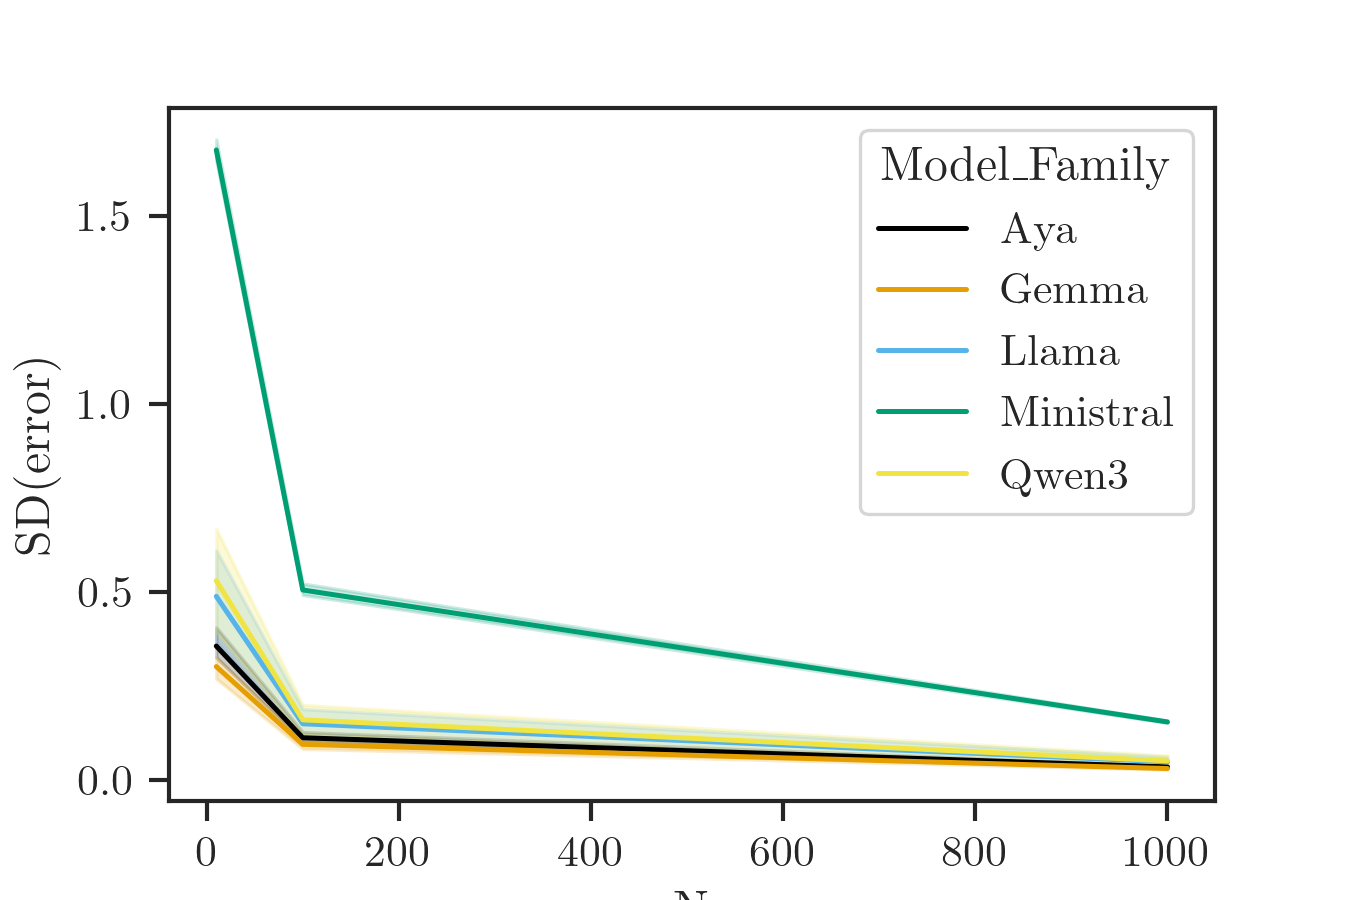
\includegraphics[width=\columnwidth]{figures/SD_error.png}
  \caption{Standard error of the sampling-based CETSCALE estimator versus
  per-condition sample size $N$, by model. Low-consensus models (e.g.,
  Ministral) incur substantially larger error at every budget.}
  \label{fig:sampling-se}
\end{figure}

\subsubsection{Decoding Bias}
\label{app:decoding-bias}

Whereas sampling noise vanishes as $N\to\infty$, 
non-default decoding introduces a systematic bias that no amount of sampling can correct, 
because temperature and top-$p$ reshape the target distribution itself. 
We quantify this deterministically. 
For each condition we recompute the exact expected composite score under a grid of temperatures 
$T\in\{0.1,0.5,1.0,1.3\}$ and
$\text{top-}p\in\{0.8,0.9,1.0\}$, 
and measure the bias relative to the model's
native ($T{=}1.0$, $\text{top-}p{=}1.0$) distribution
(Table~\ref{tab:decoding-bias}).

\begin{table*}[htbp]
  \caption{Decoding-induced bias (composite-score units) relative to the native
  distribution, aggregated over the $T\times\text{top-}p$ grid. $M_{|Bias|}$ is
  the mean absolute bias; $SD_{Bias}$ its standard deviation across the grid.
  Models sorted by Consensus.}
  \label{tab:decoding-bias}
  \centering
  \begin{small}
  \begin{sc}
  \begin{tabular}{lrrr}
  \toprule
  Model & $\mathrm{Cns}$ & $M_{|Bias|}$ & $SD_{Bias}$ \\
  \midrule
  Gemma 3-27B    & 0.95 & 0.18 & 0.25 \\
  Aya-32B        & 0.94 & 0.24 & 0.38 \\
  Llama 3.3-70B  & 0.91 & 0.59 & 0.75 \\
  Qwen3 Next-80B & 0.91 & 0.33 & 0.53 \\
  Ministral-14B  & 0.66 & 1.38 & 1.39 \\
  \bottomrule
  \end{tabular}
  \end{sc}
  \end{small}
\end{table*}

The distortion is small for high-consensus models (Gemma: $0.18$ points) but substantial for low-consensus Ministral 
($M_{|Bias|}=1.38$, reaching up to $+2.79$ points at low temperature and reversing sign at $T{=}1.3$;
Figures~\ref{fig:bias-temp}--\ref{fig:bias-topp}), comparable to the effects in
Table~\ref{tab:main-effects}. 
As with sampling noise, the bias is strongly
anti-correlated with Consensus ($r=-0.85$, $p<0.001$, $n{=}20$ conditions). 
Intuitively, the results confirm that a sharp, high-consensus PMF has almost no dispersed mass for temperature or nucleus truncation to reshape, 
whereas a flat, low-consensus PMF has its mean substantially shifted.

\begin{figure}[htbp]
  \centering
  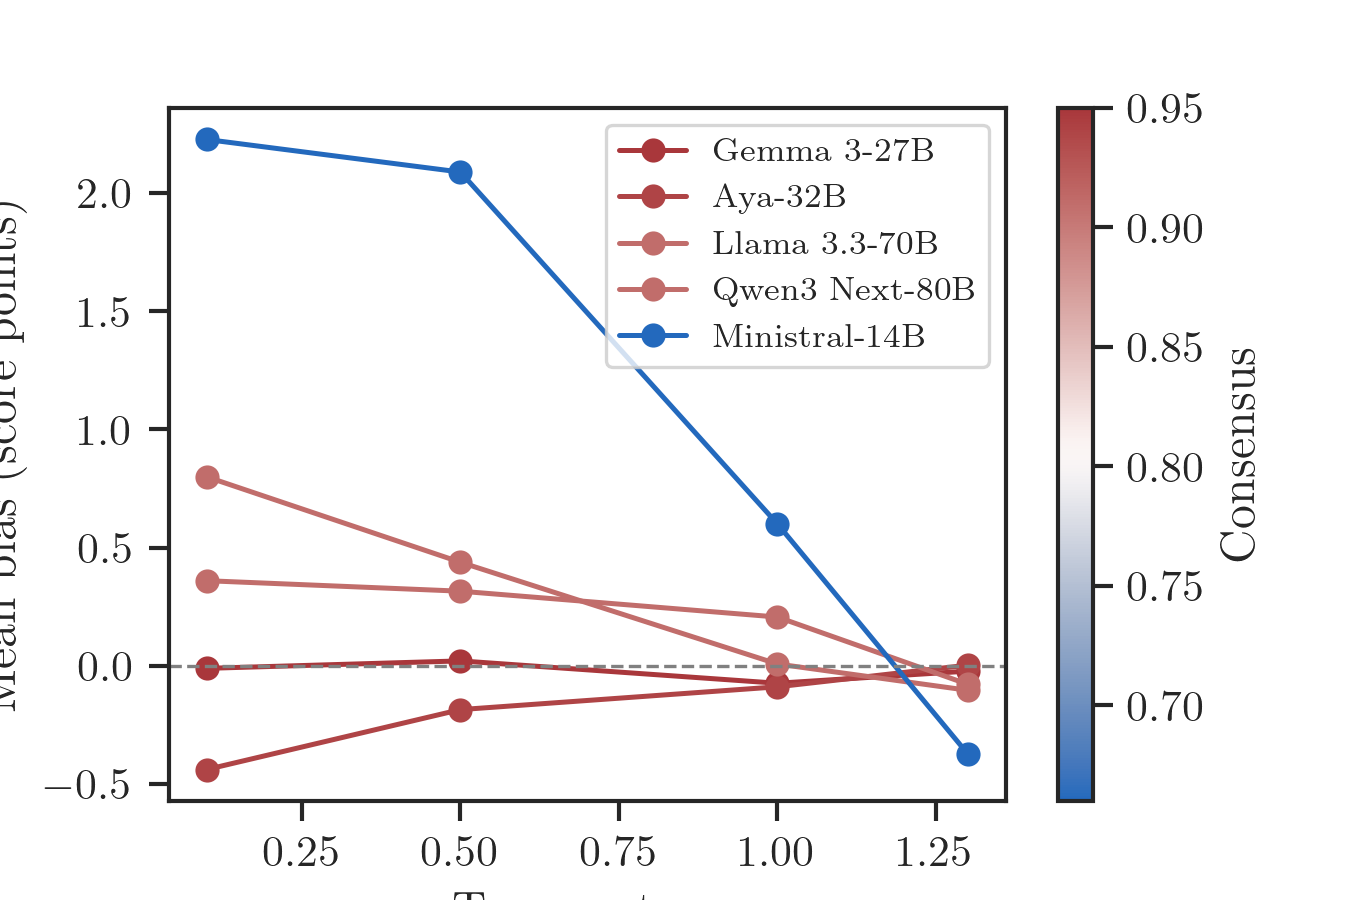
\includegraphics[width=\columnwidth]{figures/mean_bias_temperature.png}
  \caption{Mean decoding bias versus temperature, colored by Consensus.
  Low-consensus models exhibit large, sign-changing distortions.}
  \label{fig:bias-temp}
\end{figure}

\begin{figure}[htbp]
  \centering
  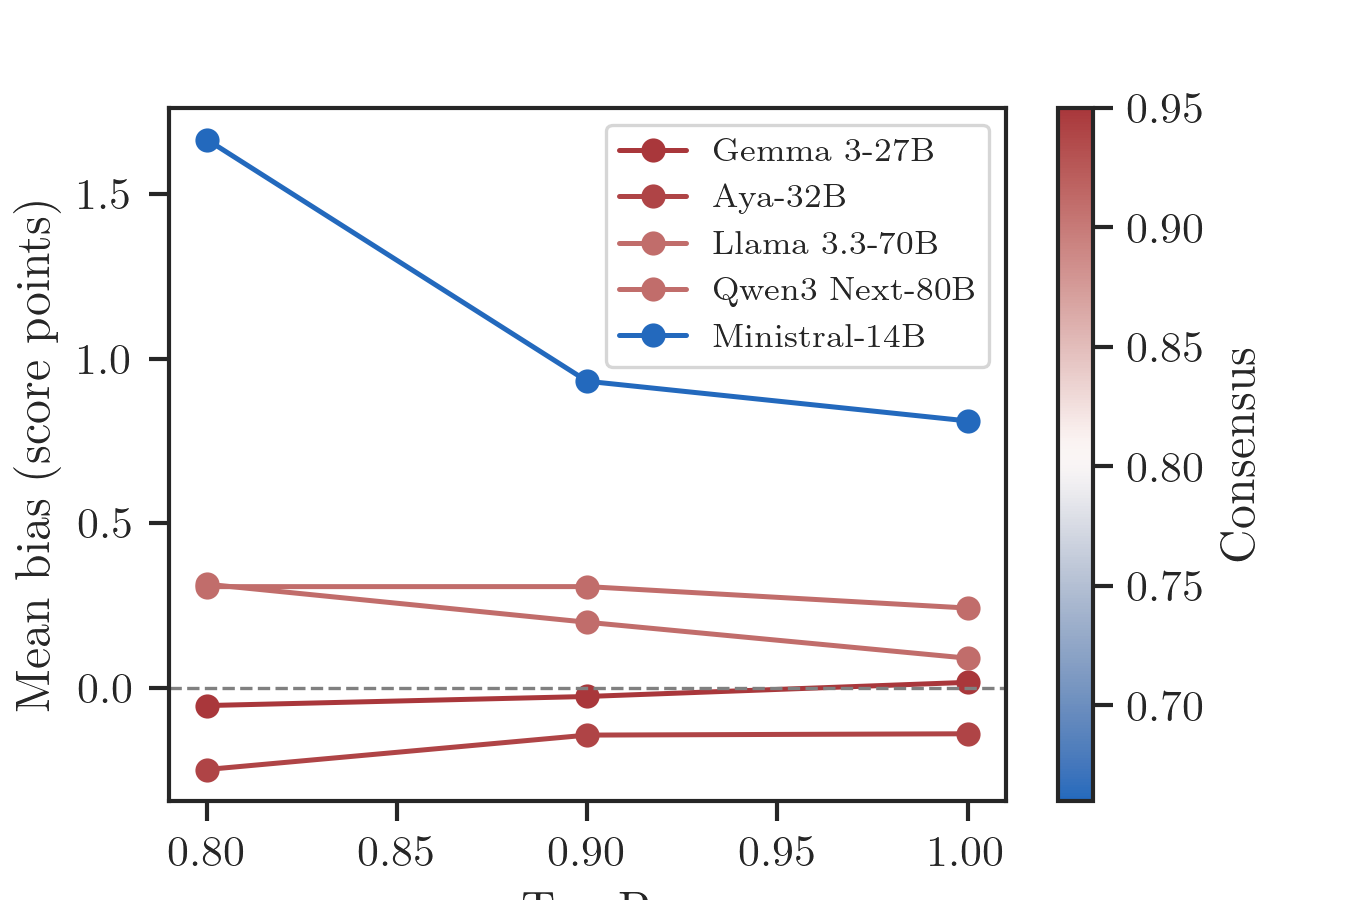
\includegraphics[width=\columnwidth]{figures/mean_bias_topp.png}
  \caption{Mean decoding bias versus top-$p$, colored by Consensus.}
  \label{fig:bias-topp}
\end{figure}




\subsection{Reliability of sampling-based estimators under ideal decoding}
\label{app:flip-analysis}


The exact-PMF framework eliminates sampling error by construction. 
To quantify what a researcher stands to lose by instead adopting the standard Monte Carlo
sampling paradigm, we ask a decision-relevant question: 
\emph{what fraction of the causal effects we report could a sampling-based study
get wrong (i.e., recover with the opposite sign) purely as an artifact of finite
sampling?}

\paragraph{Setup.}
We treat our exact effect distributions as ground truth. 
For each factorial parameter (i.e., the \textsc{Model} and \textsc{Target} main effects and every
$\textsc{Model}\times\textsc{Target}$ interaction) we compute its exact effect size $E_{\text{exact}}$ 
using the sum-to-zero contrasts consistent with
Theorem~\ref{thm:anova-consistency-main}. 
We then model a researcher who estimates the same contrast from $N$ sampled CETSCALE responses per condition.
Because items are conditionally independent (Sec.~\ref{sec:independence-assumption}),
a single composite draw has variance $\sum_{k=1}^{K}\mathrm{Var}(Y_{k})$, 
so the contrast estimator is asymptotically

$$\hat{E}\sim\mathcal{N}\!\left(E_{\text{exact}},\ \sum_{c}\alpha_c^2\,
\sigma_c^2/N\right)$$,

where $\alpha_c$ are the contrast coefficients 
and $\sigma_c^2$ is the composite variance of condition $c$. 
The \emph{flip probability} ($P_{\text{flip}}$) is the probability that the sampling estimate carries the wrong sign,

\begin{equation}
\label{eq:flip-prob}
P_{\text{flip}}
=
\Phi\!\left(
-\,\frac{\mathrm{sign}(E_{\text{exact}})\,\mathbb{E}[\hat{E}]}
{\mathrm{SD}(\hat{E})}
\right),
\end{equation}

where $\Phi$ is the standard normal CDF. 
We evaluate the realistic per-condition budgets $N\in\{10,100,1000\}$ under the default decoding setting
($T{=}1.0$, top-$p{=}1.0$), isolating the cost of sampling noise alone.

\paragraph{Results.}
Table~\ref{tab:flip-by-effectsize} bins parameters by their exact absolute effect
size (in composite-score units on the $17$--$119$ CETSCALE) and reports the mean flip probability. 
Figure~\ref{fig:p-flip} shows the full relationship between
effect size and $P_{\text{flip}}$.

\begin{table*}[htbp]
  \caption{Mean sign-flip probability of a sampling-based estimator under default
  decoding ($T{=}1.0$, top-$p{=}1.0$), stratified by exact effect size (composite-score
  units) and per-condition sample size $N$. \textit{Params} is the share of all
  factorial parameters falling in each bin.}
  \label{tab:flip-by-effectsize}
  \centering
  \begin{small}
  \begin{sc}
  \begin{tabular}{lrrrr}
  \toprule
  $|E_{\text{exact}}|$ & Params (\%) & $N{=}10$ & $N{=}100$ & $N{=}1000$ \\
  \midrule
  $[0,1)$   & 24.1 & 0.180 & 0.063 & 0.013 \\
  $[1,2)$   &  6.9 & 0.004 & 0.000 & 0.000 \\
  $[2,5)$   & 41.4 & 0.002 & 0.000 & 0.000 \\
  $[5,10)$  & 17.2 & 0.000 & 0.000 & 0.000 \\
  $\ge 10$  & 10.3 & 0.000 & 0.000 & 0.000 \\
  \bottomrule
  \end{tabular}
  \end{sc}
  \end{small}
\end{table*}

\begin{figure}[htbp]
  \centering
  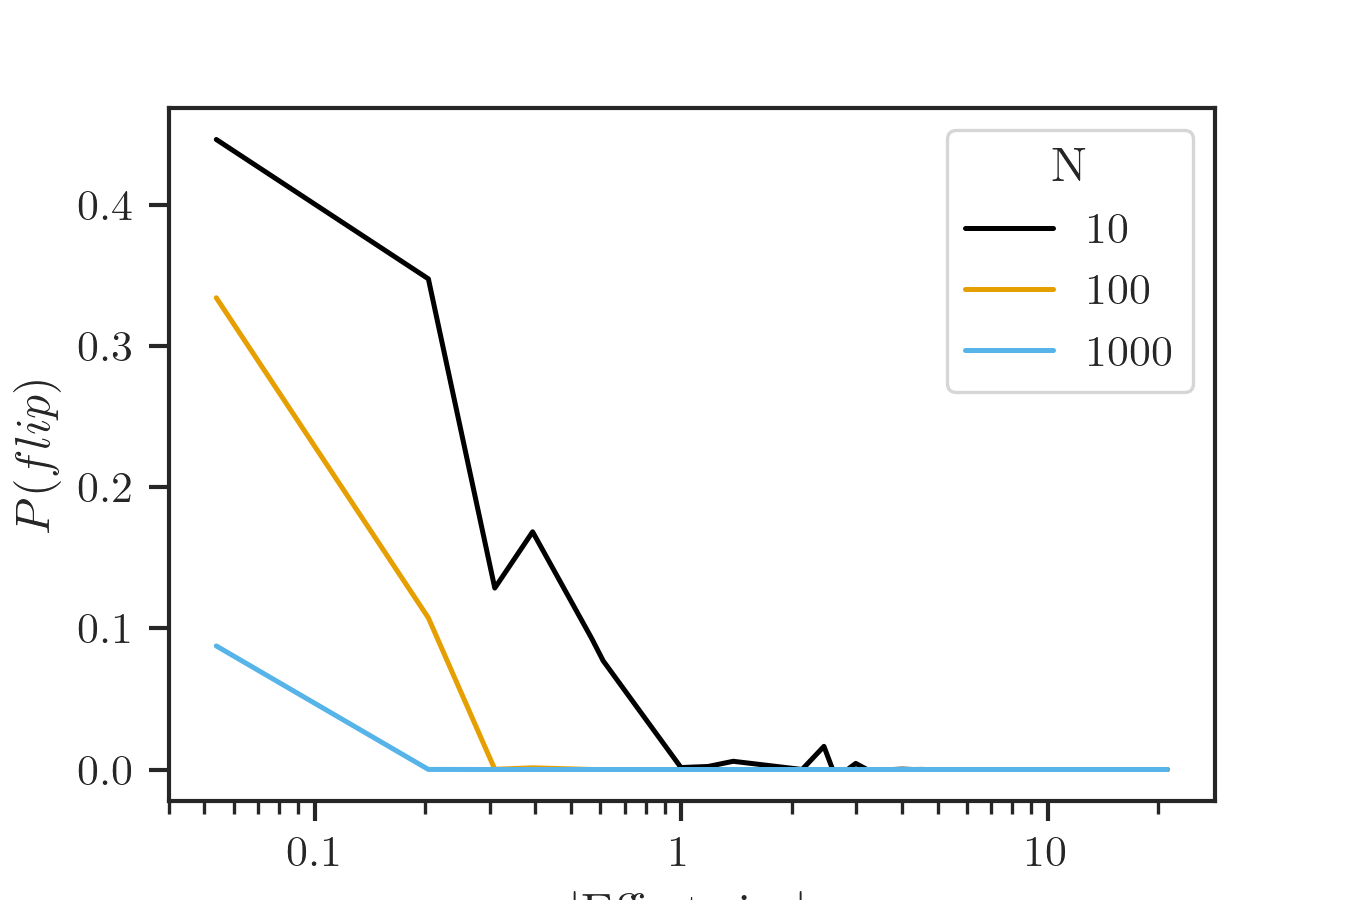
\includegraphics[width=\columnwidth]{figures/p_flip.png}
  \caption{Sign-flip probability of a sampling-based estimator as a function of
  the exact absolute effect size, for per-condition budgets
  $N\in\{10,100,1000\}$ under default decoding. Reliability degrades sharply for
  small effects and low sampling budgets, while large effects are recovered
  reliably at any $N$.}
  \label{fig:p-flip}
\end{figure}

\paragraph{Findings.}
We observe three important findings. 
First, large and moderate effects are robust. 
Every parameter with $|E_{\text{exact}}|\ge 2$ (a cumulative $68.9\%$ of all effects)
has a flip probability below $0.01$ even at the smallest budget $N{=}10$. 
A researcher would recover the sign of these effects reliably. 
Second, the risk is concentrated entirely in the small-effect regime. 
Parameters with $|E_{\text{exact}}|<1$, 
which constitute $24.1\%$ of the factorial design, 
flip $18\%$ of the time at $N{=}10$ 
and still $6.3\%$ of the time at the commonly used budget $N{=}100$. 
In our study these small effects include several substantively interesting interactions 
(e.g., the near-null Qwen3$\times$China term), 
precisely the subtle country-of-origin signals a controlled study aims to detect. 
Third, the risk decays slowly: reducing the flip rate from $18\%$ to $1.3\%$ requires a $100\times$ increase in
sample size (from $N{=}10$ to $N{=}1000$), 
reflecting the $1/\sqrt{N}$ convergence of the estimator. 
Because the exact-PMF framework attains the $N\to\infty$ limit in
a single forward pass, it removes this reliability--compute tradeoff,
and guarantees that the sign and magnitude of every reported effect are free of
sampling artifacts.












\subsection{Extending the Framework to Prompt Framing}
\label{app:prompt-framing}

A key strength of casting behavioral evaluation as a fully crossed factorial
design is extensibility: any new source of variation can be introduced as an
additional factor and analyzed through the identical distributional-ANOVA
pipeline
(Theorem~\ref{thm:anova-consistency-main},
Corollaries~\ref{cor:main-effect-anova}--\ref{cor:paired-interaction-anova}).
We demonstrate this by promoting the administration prompt to a first-class
experimental factor, $\lambda_{\text{Prompt}}$. 
This yields a new capability. 
Rather than treating prompt phrasing as a fixed background choice, 
the framework isolates its causal effect on the measured construct, quantifies how it
interacts with each model, and recovers the latent trait with framing held under
statistical control.

We construct six system-prompt framings that preserve the measurement instrument exactly, namely, all retain the 1--7 scale, the agreement polarity, and the digit-only response schema, and hold every CETSCALE item verbatim. 
Only the surrounding framing wording varies (Table~\ref{tab:prompt-variants}). 
We evaluate a fully crossed $\textsc{Model}\times\textsc{Target}\times\textsc{Prompt}$ design over three models spanning the consensus and ethnocentrism ranges observed in the main study (Gemma~3~27B, Aya~Expanse~32B, Ministral~14B), four target countries, and the six framings, for $3\times4\times6\times17=1{,}224$ exact item-level PMFs.

\begin{table*}[htbp]
  \caption{Prompt framing variants. All preserve the 1--7 scale, agreement
  polarity, and digit-only response schema; every CETSCALE item is held verbatim.}
  \label{tab:prompt-variants}
  \centering
  \begin{small}
  \begin{tabular}{@{}p{3.4cm}p{8.6cm}@{}}
    \toprule
    \textbf{Variant} & \textbf{Framing} \\
    \midrule
    v0\_original & Consumer market-research persona; explicit 7-point scale; digit only. \\
    v1\_participant & Survey-participant framing; agreement scale 1--7; single digit only. \\
    v2\_concise & Minimal instruction; rate 1--7; output only the number. \\
    v3\_instructional & Task-style instruction; scale 1 (disagree) to 7 (agree); digit 1--7 only. \\
    v4\_roleplay & Everyday-shopper roleplay; 7 = agree, 1 = disagree; digit only. \\
    v5\_original\_no\_whitespace & v0 wording with whitespace/formatting normalized. \\
    \bottomrule
  \end{tabular}
  \end{small}
\end{table*}

\paragraph{Isolated effects under the three-factor design.}
Table~\ref{tab:prompt-effects} reports the full decomposition: 
The grand-mixture baseline $\mu_\emptyset$, the isolated main effects for all three factors, and the
three families of two-way interactions
($\textsc{Model}\times\textsc{Target}$, $\textsc{Model}\times\textsc{Prompt}$,
$\textsc{Target}\times\textsc{Prompt}$). 
Each row is an exact effect distribution summarized by mean shift ($\mathbb{E}$), predictive dispersion (SD),
signal-to-noise ratio (SNR), and discrete probability of direction (dPD).

Three capabilities of the framework are visible directly in Table~\ref{tab:prompt-effects}. 
First, the country-of-origin signal is recovered with framing controlled. 
The $\textsc{Target}$ main effects reproduce the pattern of the main study (Canada $+4.7$, China $-6.4$, France $-0.4$, USA $+2.1$), and every $\textsc{Target}\times\textsc{Prompt}$ interaction is small (all
$|\mathbb{E}|<1.5$, SNR $<0.4$, dPD near chance). 

Second, prompt framing is quantified as its own causal effect. 
The $\textsc{Prompt}$ main effect spans roughly $13$ composite-score points ($+6.9$ for v5 to $-6.7$ for v2), giving a direct, exact measurement of how administration framing shifts the construct
level. 

Third, model-specific framing sensitivity becomes measurable. 
The $\textsc{Model}\times\textsc{Prompt}$ block shows Gemma~3~27B interacting weakly with framing (all $|\mathbb{E}|<3.9$, SNR $<0.5$), 
whereas Aya~32B and Ministral~14B interact strongly (Aya$\times$v2 SNR $2.2$; Ministral$\times$v0
SNR $1.6$). 
Consistent with these interactions, the prompt-controlled $\textsc{Model}$ main effects recover the trait ordering of the main study, with Aya~32B highest ($+9.1$), Ministral~14B intermediate ($+4.0$), and Gemma~3~27B lowest ($-13.0$). 
The reduced magnitudes relative to Table~\ref{tab:coefficient-table-marginal} reflect the three-model subset and its distinct grand mean ($\mu_\emptyset=62.3$).


% ==========================================
% TABLE PART 1
% ==========================================
\begin{table*}[htbp]
  \caption{Full three-factor effect decomposition (Part 1 of 2: Main effects and Model $\times$ Target). Rows are isolated effect distributions summarized by mean shift ($\mathbb{E}$), predictive dispersion (SD), signal-to-noise ratio (SNR), and discrete probability of direction (dPD).}
  \label{tab:prompt-effects}
  \centering
  \begin{small}
  \begin{sc}
  \begin{tabular}{lrrll}
  \toprule
  Parameter & $\mathbb{E}$ & $\mathrm{SD}$ & $\mathrm{SNR}$ & $\mathrm{dPD}$ \\
  \midrule
  $\mu_{\emptyset}$ & 62.34 & 13.49 &  &  \\
  \midrule
  Aya-32B        &   9.08 & 12.67 & 0.72 & 0.76 \\
  Gemma 3-27B    & -13.03 & 11.74 & 1.11 & 0.90 \\
  Ministral-14B  &   3.96 &  9.61 & 0.41 & 0.70 \\
  \midrule
  Canada &   4.74 & 5.24 & 0.90 & 0.93 \\
  China  &  -6.38 & 6.08 & 1.05 & 0.97 \\
  France &  -0.44 & 4.78 & 0.09 & 0.48 \\
  USA    &   2.08 & 5.43 & 0.38 & 0.44 \\
  \midrule
  v0\_original       &   6.74 & 10.16 & 0.66 & 0.64 \\
  v1\_participant    &  -0.17 &  7.22 & 0.02 & 0.58 \\
  v2\_concise        &  -6.68 &  9.73 & 0.69 & 0.82 \\
  v3\_instructional  &  -4.08 &  7.76 & 0.53 & 0.62 \\
  v4\_roleplay       &  -2.67 &  6.94 & 0.38 & 0.68 \\
  v5\_no\_whitespace &   6.86 &  9.32 & 0.74 & 0.74 \\
  \midrule
  Aya-32B $\times$ Canada       &  0.31 & 2.14 & 0.15 & 0.35 \\
  Aya-32B $\times$ China        &  0.36 & 4.01 & 0.09 & 0.51 \\
  Aya-32B $\times$ France       &  0.08 & 3.33 & 0.03 & 0.53 \\
  Aya-32B $\times$ USA          & -0.75 & 3.47 & 0.22 & 0.48 \\
  \midrule
  Gemma 3-27B $\times$ Canada   &  2.14 & 3.28 & 0.65 & 0.62 \\
  Gemma 3-27B $\times$ China    & -4.40 & 9.86 & 0.45 & 0.59 \\
  Gemma 3-27B $\times$ France   & -1.83 & 5.38 & 0.34 & 0.55 \\
  Gemma 3-27B $\times$ USA      &  4.09 & 3.47 & 1.18 & 0.88 \\
  \midrule
  Ministral-14B $\times$ Canada & -2.45 & 3.08 & 0.80 & 0.77 \\
  Ministral-14B $\times$ China  &  4.04 & 4.52 & 0.89 & 0.82 \\
  Ministral-14B $\times$ France &  1.74 & 2.48 & 0.70 & 0.74 \\
  Ministral-14B $\times$ USA    & -3.34 & 4.10 & 0.81 & 0.77 \\
  \bottomrule
  \end{tabular}
  \end{sc}
  \end{small}
\end{table*}

% ==========================================
% TABLE PART 2
% ==========================================
\begin{table*}[htbp]
  \caption{Full three-factor effect decomposition (Part 2 of 2: Model $\times$ Prompt and Target $\times$ Prompt interactions).}
  \label{tab:prompt-effects-p2}
  \centering
  \begin{small}
  \begin{sc}
  \begin{tabular}{lrrll}
  \toprule
  Parameter & $\mathbb{E}$ & $\mathrm{SD}$ & $\mathrm{SNR}$ & $\mathrm{dPD}$ \\
  \midrule
  Aya-32B $\times$ v0        &  9.20 & 14.27 & 0.64 & 0.66 \\
  Aya-32B $\times$ v1        & -3.14 &  7.48 & 0.42 & 0.66 \\
  Aya-32B $\times$ v2        & -9.64 &  4.36 & 2.21 & 1.00 \\
  Aya-32B $\times$ v3        & -5.12 &  6.00 & 0.85 & 0.84 \\
  Aya-32B $\times$ v4        &  0.13 &  8.15 & 0.02 & 0.51 \\
  Aya-32B $\times$ v5        &  8.57 & 12.80 & 0.67 & 0.66 \\
  \midrule
  Gemma 3-27B $\times$ v0    & -0.99 &  5.35 & 0.18 & 0.47 \\
  Gemma 3-27B $\times$ v1    & -1.48 &  3.10 & 0.48 & 0.64 \\
  Gemma 3-27B $\times$ v2    &  3.89 &  2.14 & 1.82 & 0.97 \\
  Gemma 3-27B $\times$ v3    &  0.90 &  2.80 & 0.32 & 0.67 \\
  Gemma 3-27B $\times$ v4    & -0.11 &  3.41 & 0.03 & 0.44 \\
  Gemma 3-27B $\times$ v5    & -2.20 &  4.84 & 0.46 & 0.56 \\
  \midrule
  Ministral-14B $\times$ v0  & -8.22 &  5.09 & 1.61 & 1.00 \\
  Ministral-14B $\times$ v1  &  4.62 &  3.39 & 1.36 & 0.99 \\
  Ministral-14B $\times$ v2  &  5.75 &  3.77 & 1.53 & 0.95 \\
  Ministral-14B $\times$ v3  &  4.23 &  3.80 & 1.11 & 0.96 \\
  Ministral-14B $\times$ v4  & -0.01 &  3.81 & 0.00 & 0.64 \\
  Ministral-14B $\times$ v5  & -6.37 &  4.41 & 1.44 & 0.96 \\
  \midrule
  Canada $\times$ v0 & -1.04 & 2.88 & 0.36 & 0.80 \\
  Canada $\times$ v1 &  0.26 & 2.58 & 0.10 & 0.59 \\
  Canada $\times$ v2 &  1.28 & 3.36 & 0.38 & 0.57 \\
  Canada $\times$ v3 &  0.01 & 2.66 & 0.00 & 0.42 \\
  Canada $\times$ v4 & -0.22 & 2.27 & 0.10 & 0.36 \\
  Canada $\times$ v5 & -0.29 & 3.17 & 0.09 & 0.54 \\
  \midrule
  China $\times$ v0  &  0.46 & 3.56 & 0.13 & 0.65 \\
  China $\times$ v1  &  0.75 & 3.30 & 0.23 & 0.37 \\
  China $\times$ v2  & -1.45 & 4.88 & 0.30 & 0.46 \\
  China $\times$ v3  & -0.35 & 3.52 & 0.10 & 0.58 \\
  China $\times$ v4  &  0.76 & 3.64 & 0.21 & 0.45 \\
  China $\times$ v5  & -0.17 & 4.16 & 0.04 & 0.56 \\
  \midrule
  France $\times$ v0 &  0.42 & 3.43 & 0.12 & 0.37 \\
  France $\times$ v1 & -0.93 & 3.37 & 0.27 & 0.62 \\
  France $\times$ v2 & -0.21 & 3.38 & 0.06 & 0.46 \\
  France $\times$ v3 &  1.19 & 4.08 & 0.29 & 0.59 \\
  France $\times$ v4 & -0.55 & 3.44 & 0.16 & 0.41 \\
  France $\times$ v5 &  0.07 & 3.73 & 0.02 & 0.42 \\
  \midrule
  USA $\times$ v0    &  0.16 & 2.39 & 0.06 & 0.45 \\
  USA $\times$ v1    & -0.09 & 2.17 & 0.04 & 0.44 \\
  USA $\times$ v2    &  0.38 & 3.14 & 0.12 & 0.46 \\
  USA $\times$ v3    & -0.84 & 2.43 & 0.35 & 0.57 \\
  USA $\times$ v4    &  0.01 & 2.20 & 0.00 & 0.46 \\
  USA $\times$ v5    &  0.39 & 2.91 & 0.13 & 0.48 \\
  \bottomrule
  \end{tabular}
  \end{sc}
  \end{small}
\end{table*}
